\chapter{Experimental Procedure and Results of Polymerase Modeling} % (fold)
\label{cha:experimental_results_of_polymerase_modeling}
The procedure for performing an experiment with the model for polymerase directionality evolution consists of constructing an environment for the model to operate on, then setting the model running for a set number of time steps. Various parameters of the simulation are reported at set intervals during the run. Because a number of the dynamical systems in the model depend on randomly generated numbers, each experiment was carried out in 10 copies to smooth fluctuations, and all of the values reported represent a numerical average of all 10 runs. All plots were generated using the R software package.

The dynamics included in the model for polymerase directionality should generate scale free results. That is, the evolution of traits should show the same dynamics regardless of population size or genome length. In this model, the only trait capable of evolving is polymerase rate, so in order to verify that the dynamics were indeed scale free, the first experiments carried out were designed to investigate simple dynamics of polymerase rate evolution over a range of scales. One experiment consisted of starting populations of 10 organisms and a maximum population (environmental carrying capacity) of 1000 organisms combined with 4 different genome lengths as described in table~\ref{tab:scale_length}.

\begin{table}
	\begin{center}
		\begin{tabular}[c]{ c | l | l | l | l }
			Experiment & Temp. ($t$) & Starting Pop. & Max Pop. & Genome Length \\
			\hline
			\#1 & 0.40 & 10 & 1000 & 10 \\
			\#2 & 0.40 & 10 & 1000 & 100 \\
			\#3 & 0.40 & 10 & 1000 & 1000 \\
			\#4 & 0.40 & 10 & 1000 & 10000 \\
		\end{tabular}
		\caption{Determining genome length scale effects.}
		\label{tab:scale_length}
	\end{center}
\end{table}

In order to avoid a founder bias with regards to polymerase rate, in each experiment the ten organisms in each seed population consisted of one organism of each of the ten possible polymerase rates. The simulation temperature of 0.40 was chosen because it results in a significant amount of error, and therefore introduced variability, during growth but is not a high enough temperature that certain other temperature effects begin to alter growth and evolution. The results from this experiment are plotted in figure~\ref{fig:scale_length}.

\begin{figure}[h]
	\centering
		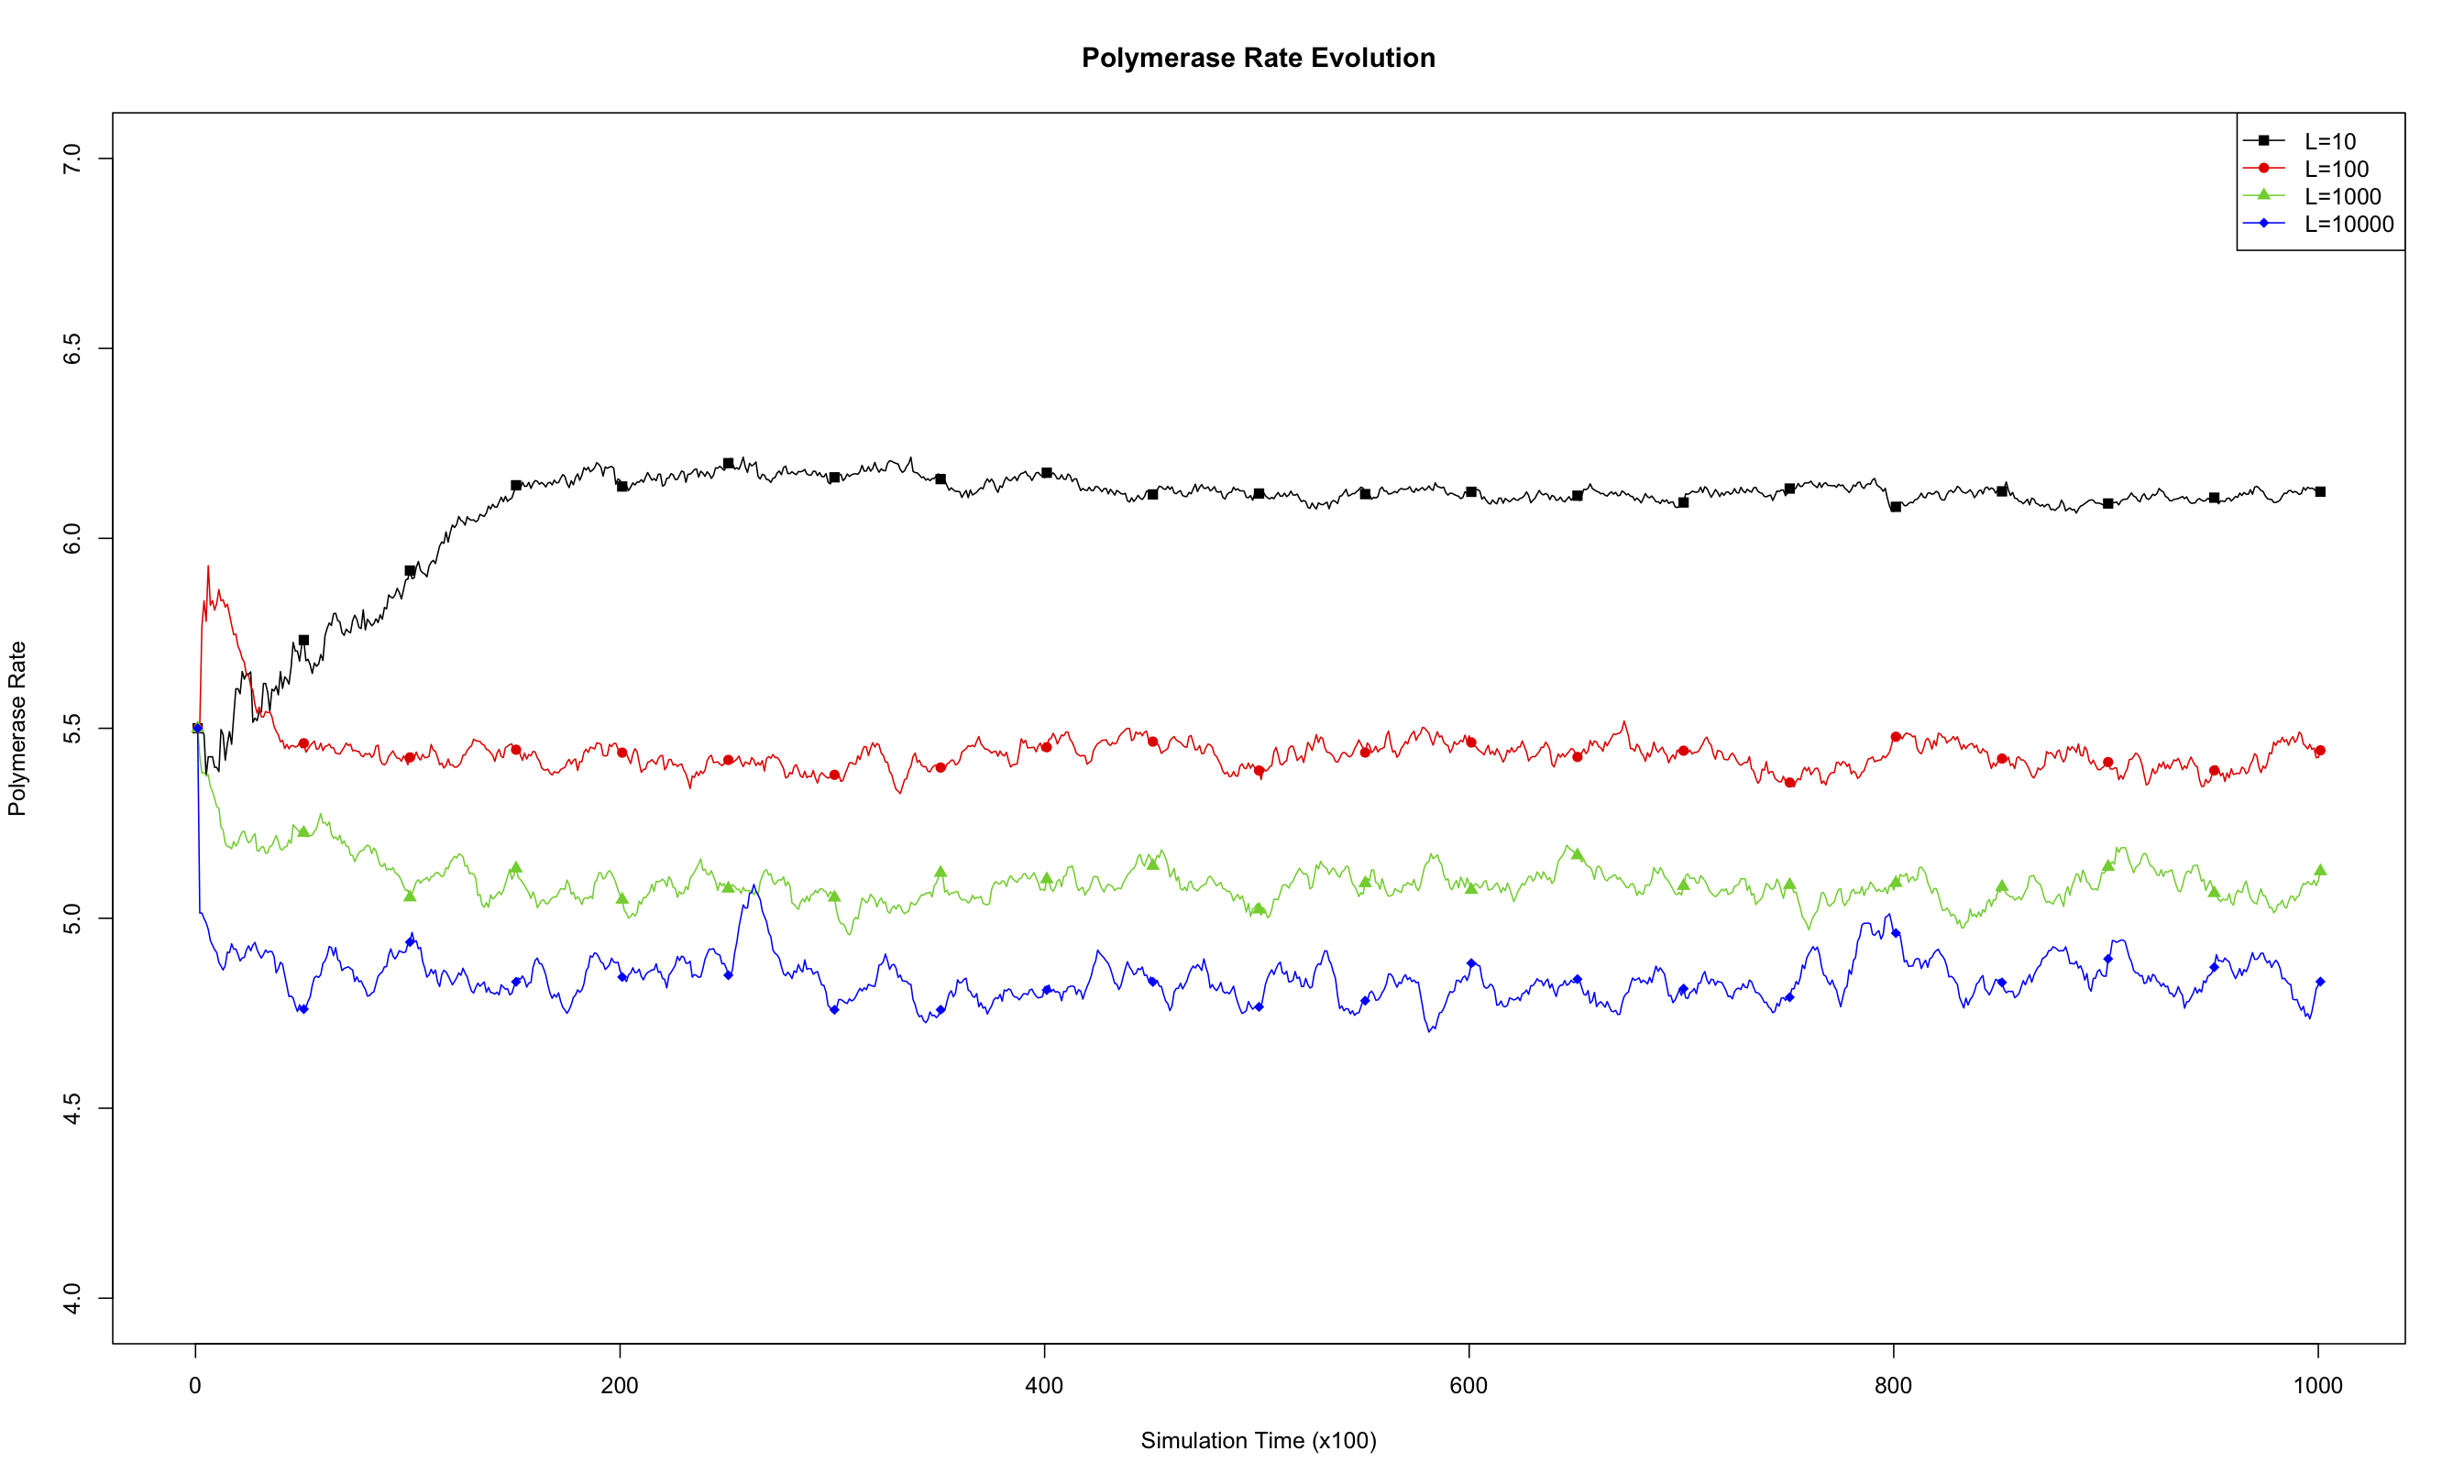
\includegraphics[width=\textwidth]{scale_length}
	\caption{\textbf{Effects of Genome Length on Polymerase Rate Evolution.} The average polymerase rate for the entire simulation population is plotted against simulation time steps (each unit on the abscissa is equivalent to 100 simulation time steps). The organisms each had genomes of length 10, 100, 1000, or 10000.}
	\label{fig:scale_length}
\end{figure}

Second, a set of experiments were carried out to investigate the effect of population size on the evolution of polymerase rate. In this experiment, the genome length of the organisms in each environment was held constant at 1000, the starting population was set to 10, and the maximum population was set to either 100, 1000, 10000, or 100000. As in the first set of experiments, the starting population in each environment was seeded with organisms with polymerase rates evenly distributed in the range 1-10 and the simulation temperature was set to 0.40. Table~\ref{tab:scale_num} summarizes these experiments.

\begin{table}
	\begin{center}
		\begin{tabular}[c]{ c | l | l | l | l }
			Experiment & Temp. ($t$) & Starting Pop. & Max Pop. & Genome Length \\
			\hline
			\#5 & 0.40 & 10 & 100 & 1000 \\
			\#6 & 0.40 & 10 & 1000 & 1000 \\
			\#7 & 0.40 & 10 & 10000 & 1000 \\
			\#8 & 0.40 & 10 & 100000 & 1000 \\
		\end{tabular}
		\caption{Determining size scale effects.}
		\label{tab:scale_num}
	\end{center}
\end{table}

Figure~\ref{fig:scale_num} is a plot of the average polymerase rate of the population in each environment against the simulation time. Based on these initial experiments, it was decided that a maximum population size of 1000 with a genome length of 1000 could serve as an adequate representative of the dynamics over the range of possible values. These values were chosen because they also keep the size of the simulations reasonable with regards to the amount of computational time required to run each simulation, since the run time of the simulations scale with the population size and organisms with longer genomes require more time-steps to achieve the same number of doublings as organisms with shorter genomes.

\begin{figure}[h]
	\centering
		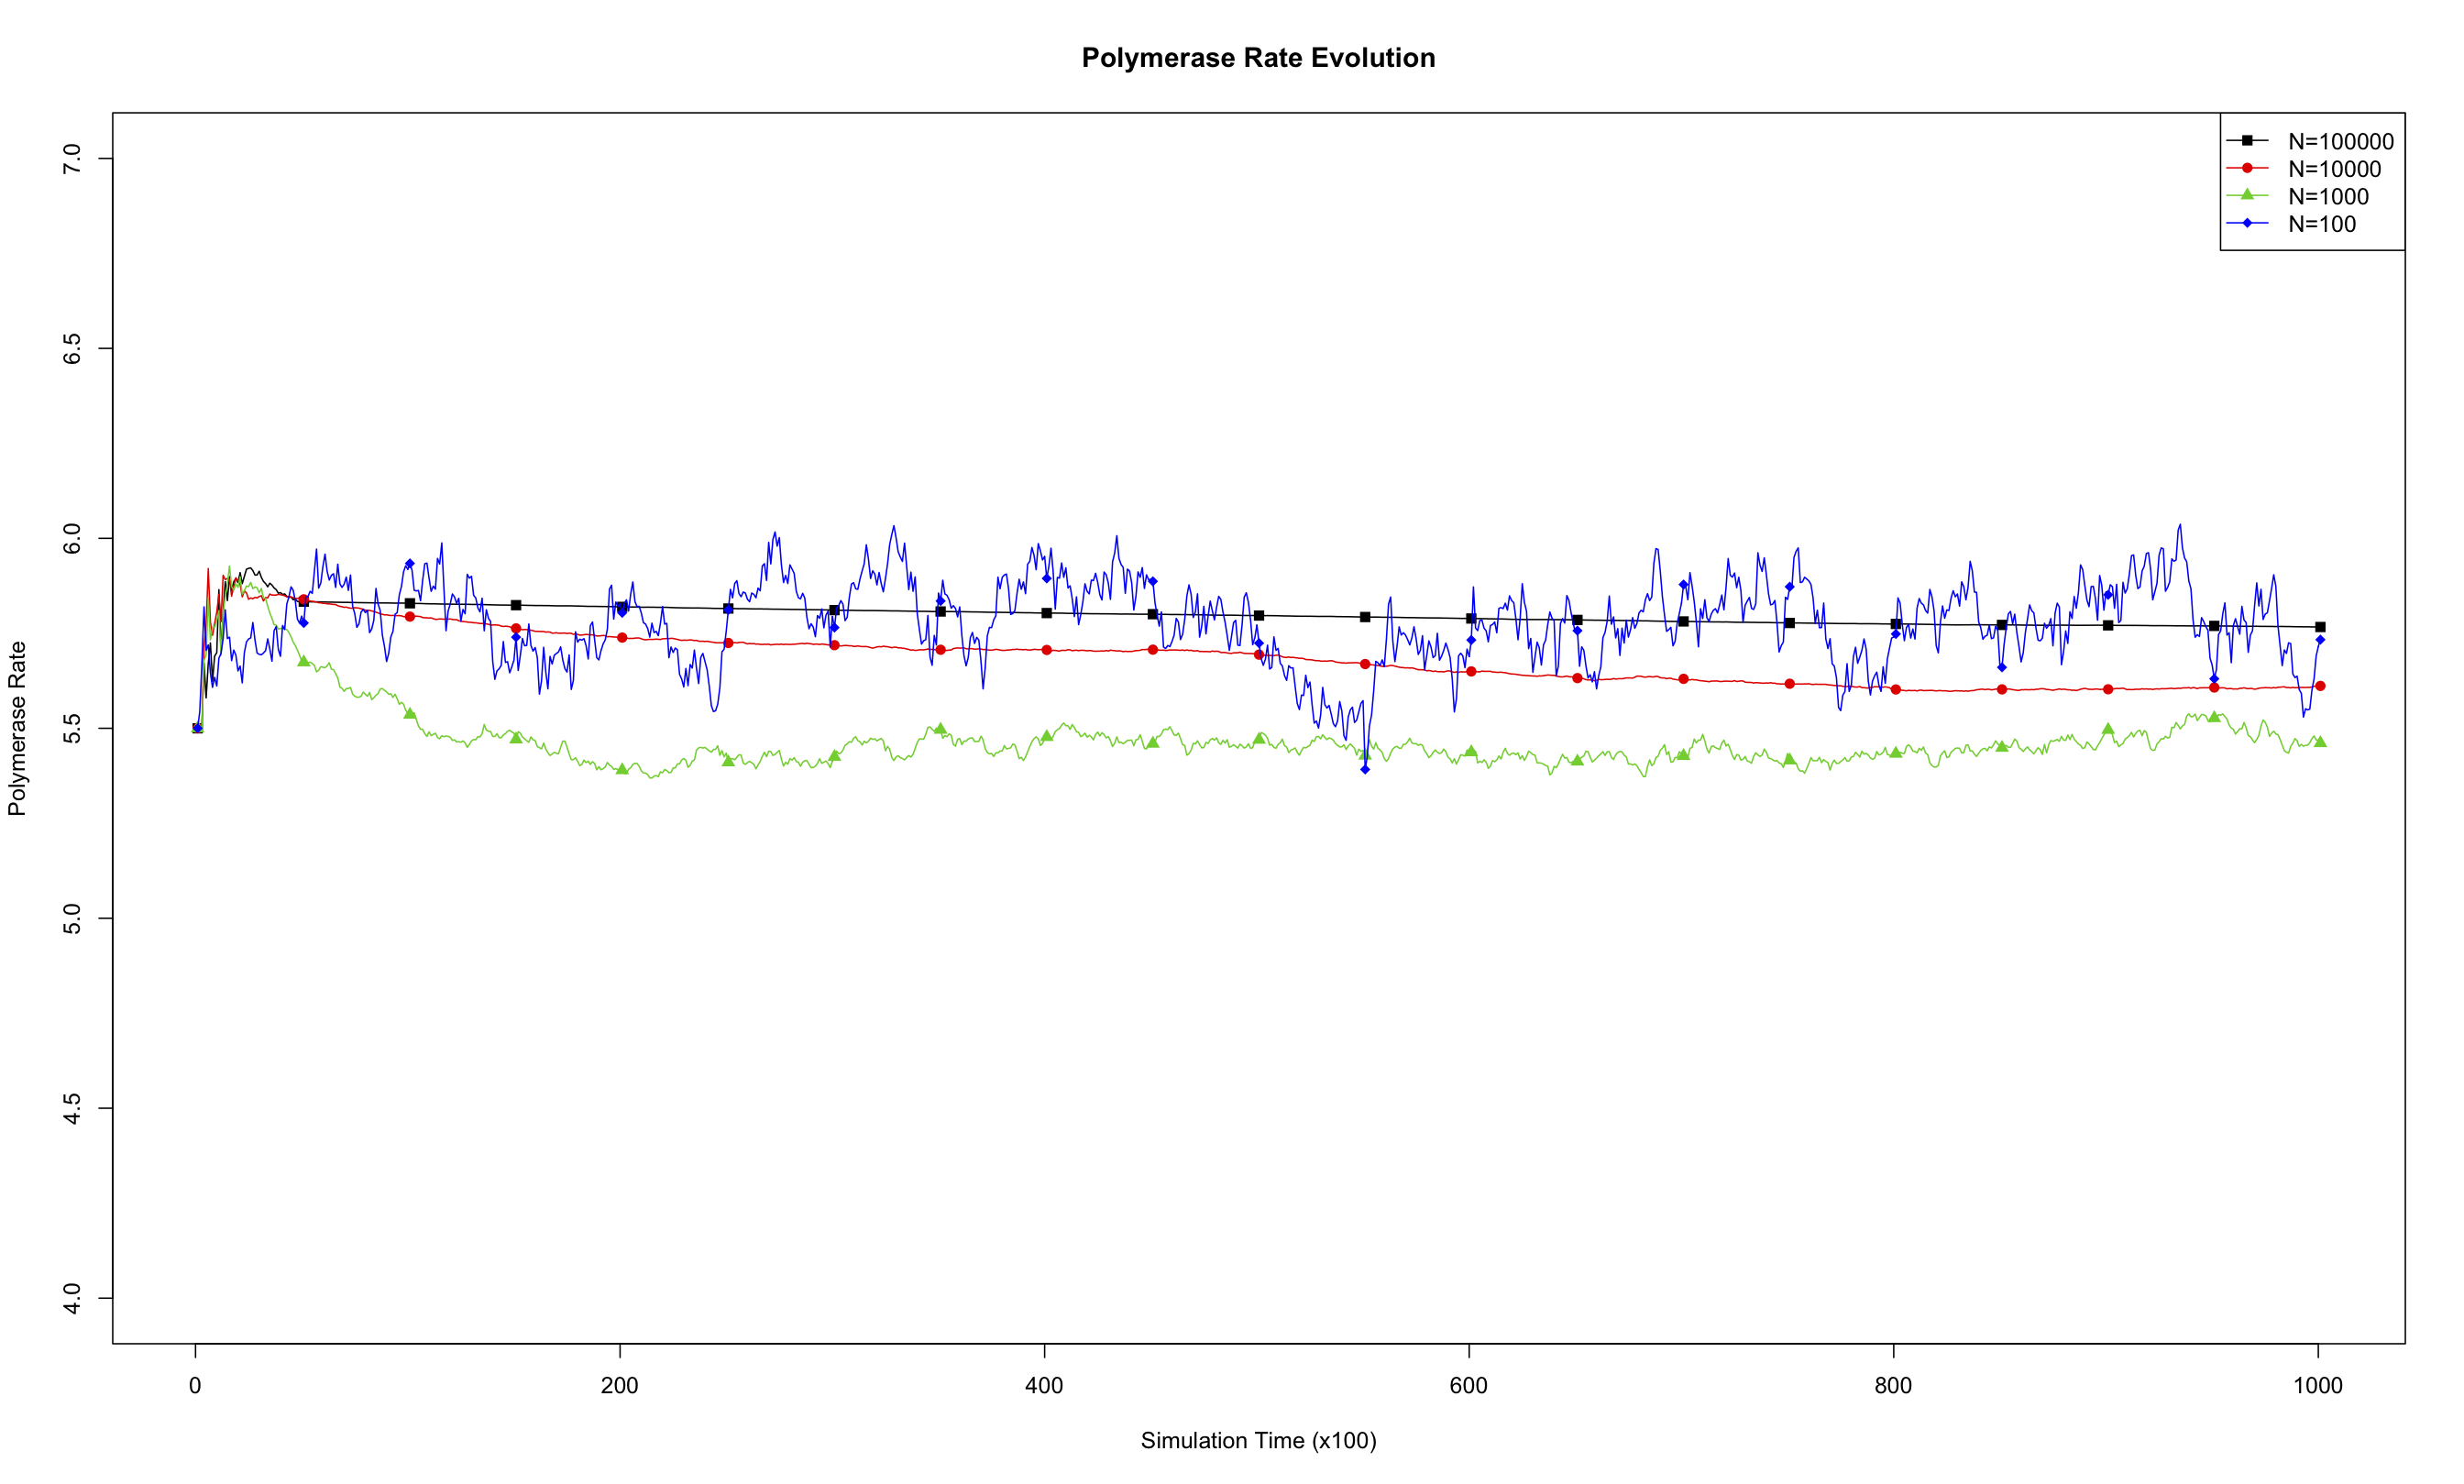
\includegraphics[width=\textwidth]{scale_num}
	\caption{\textbf{Effects of Environmental Carrying Capacity on Polymerase Rate Evolution.} The average polymerase rate for the entire simulation population is plotted against simulation time steps (each unit on the abscissa is equivalent to 100 simulation time steps). The organisms each had a genome length of 1000, and the environments had a maximum capacity ($N$) of 100, 1000, 10000, or 100000 organisms.}
	\label{fig:scale_num}
\end{figure}

Finally, in order to validate the model and how reasonably it simulates the observed growth dynamics of biological organisms, a set of experiments were carried out starting with small populations of 10 organisms, as before, and following their growth at different temperatures. The first two sets of experiments were only carried out with forward polymerizing organisms. To be sure that model organisms with reverse, $3'\to5'$, polymerases had growth dynamics similar to forward polymerizing organisms, these experiments were carried out using both types of organisms. Table~\ref{tab:temp_incr} summarizes the parameters used for these experiments.

\begin{table}
	\begin{center}
		\begin{tabular}[c]{ c | l | l | l | l }
			Experiment & Temp. ($t$) & Max Pop. & Genome Length & Directionality \\
			\hline
			& 0.10 & & &\\
			& 0.30 & & &\\
			\#9-13 & 0.40 & 1000 & 1000 & forward \\
			& 0.50 & & &\\
			& 0.60 & & &\\
			\hline
			& 0.10 & & &\\
			& 0.30 & & &\\
			\#14-18 & 0.40 & 1000 & 1000 & reverse \\
			& 0.50 & & &\\
			& 0.60 & & &\\
		\end{tabular}
		\caption{Growth dynamics at various temperatures.}
		\label{tab:temp_incr}
	\end{center}
\end{table}

For each experiment, the population was plotted against simulation time in figure~\ref{fig:temp_incr_num} and the average polymerase rate of all the organisms in each environment is plotted in figure~\ref{fig:temp_incr_rate}. Values for the forward polymerizing organisms are indicated with closed circles and values for the reverse polymerizing organisms are indicated with open circles.

\begin{figure}[h]
	\centering
		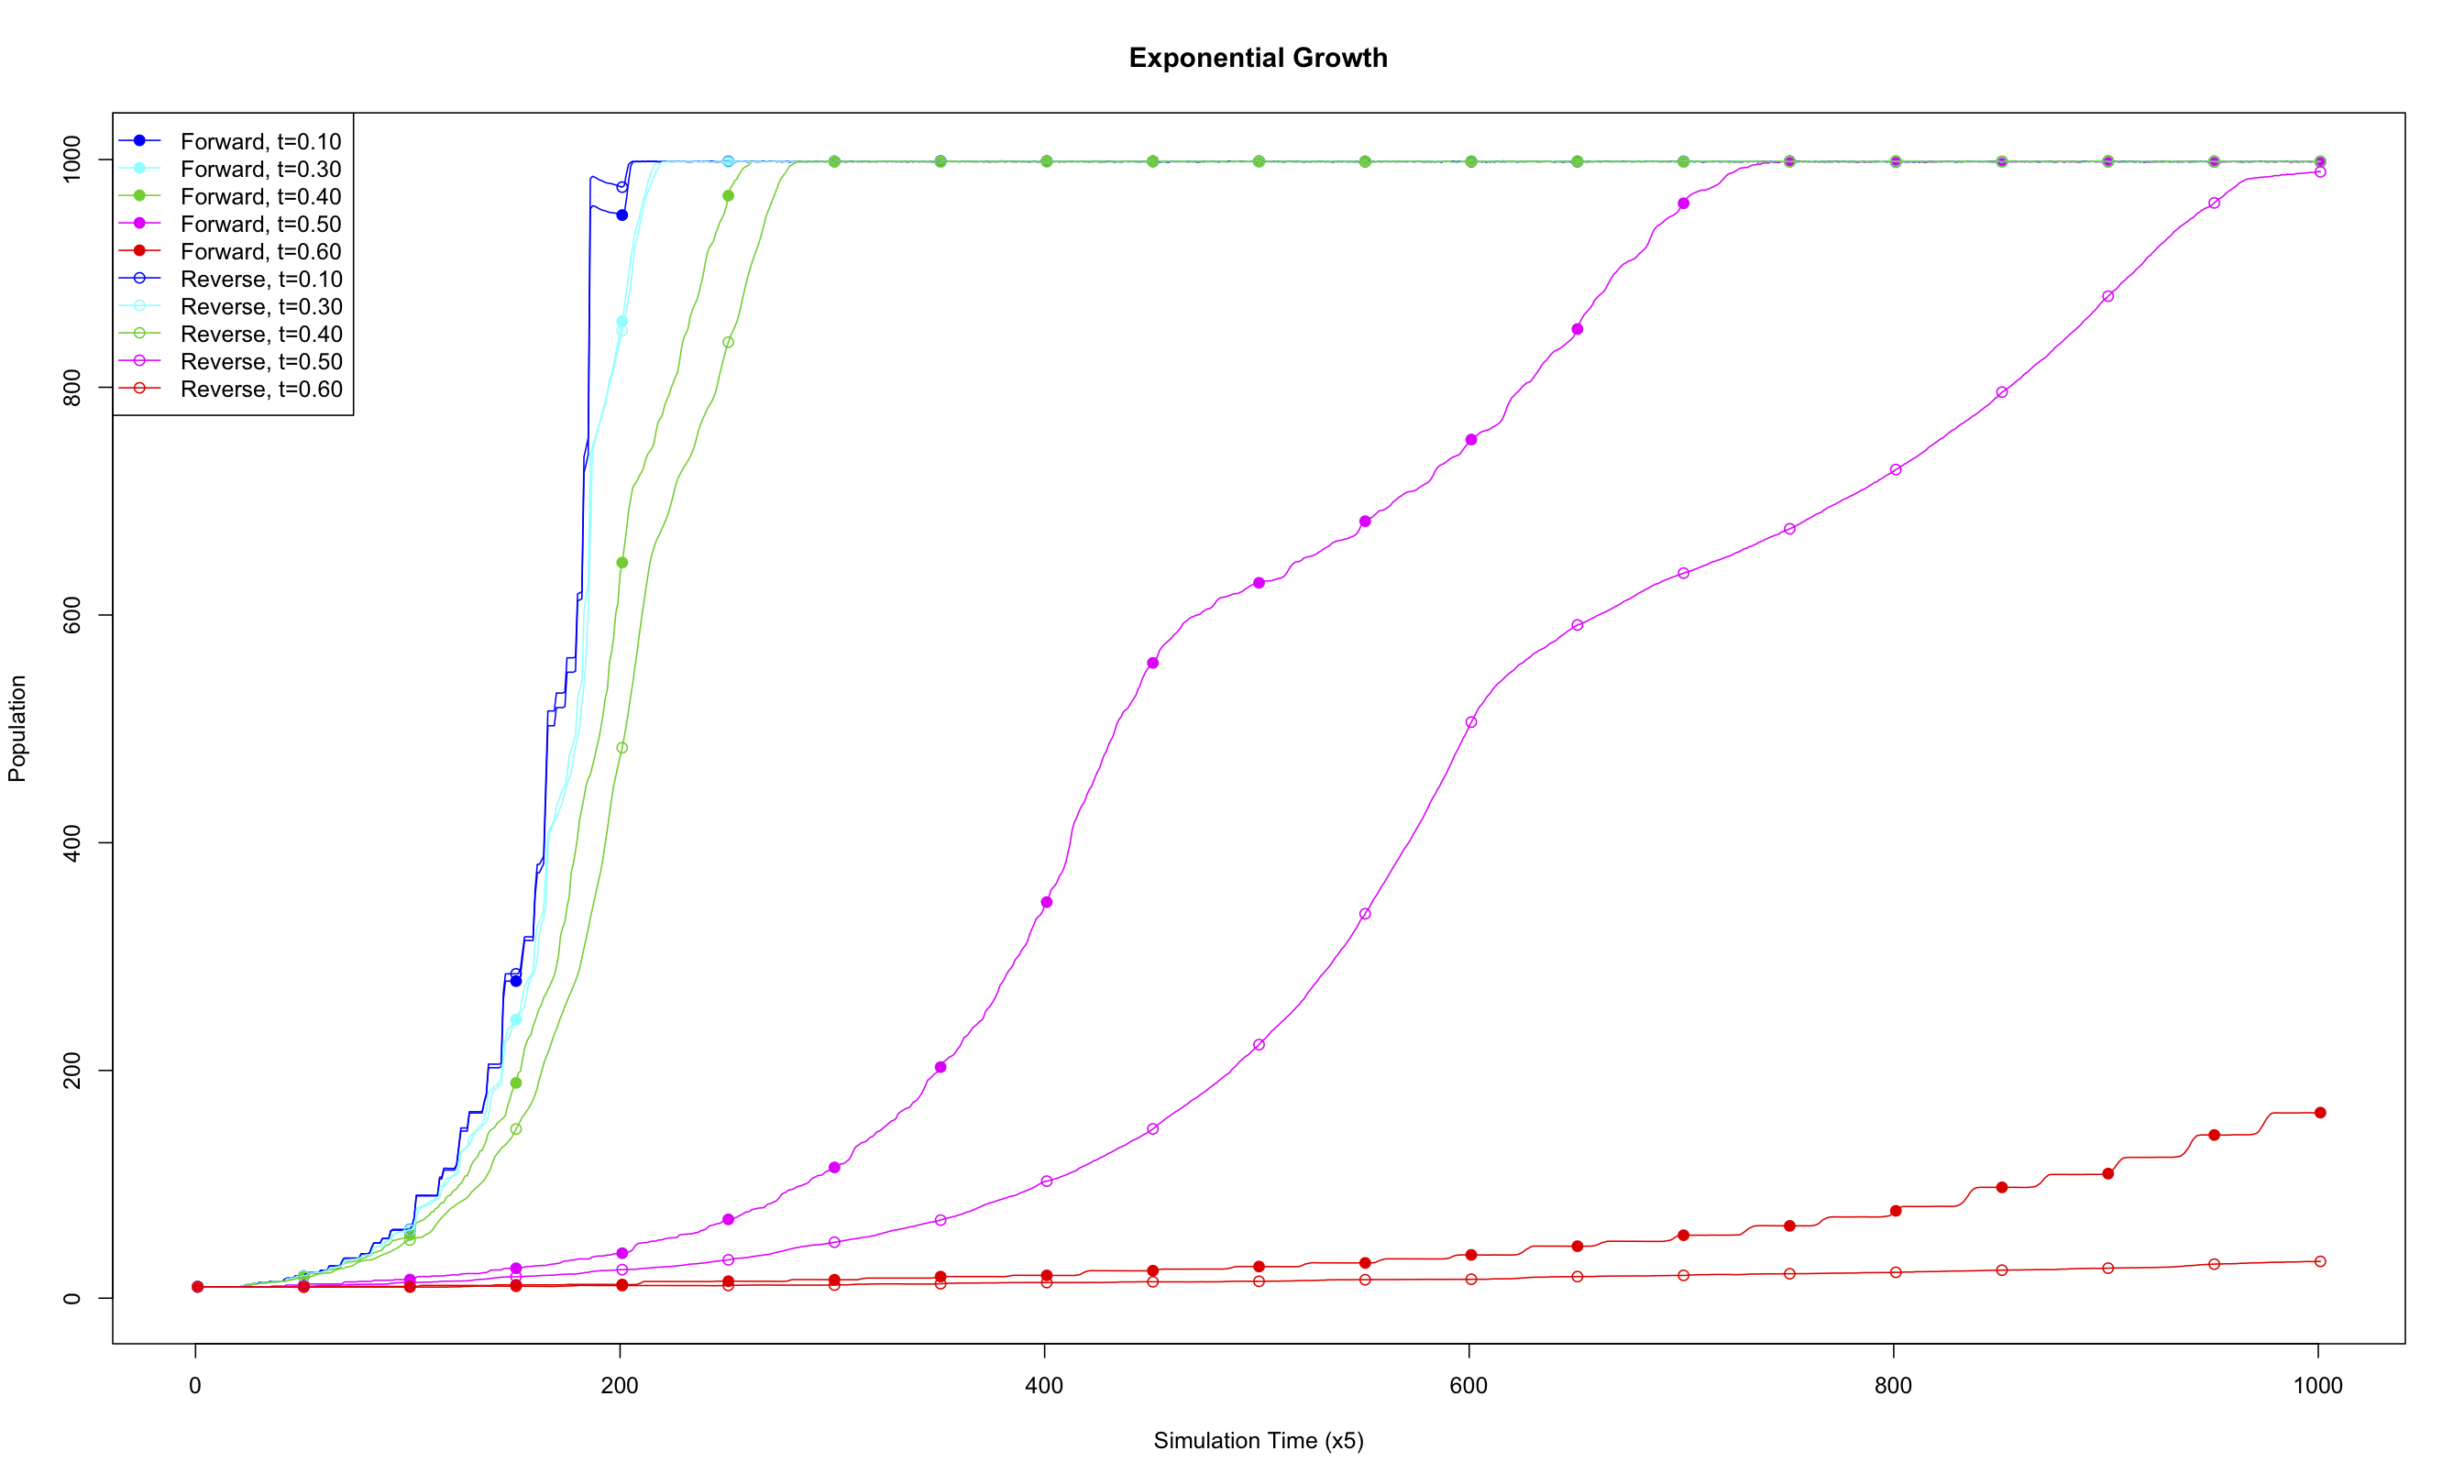
\includegraphics[width=\textwidth]{temp_incr_num}
	\caption{\textbf{Growth of model organisms at various temperatures.} The population size at each time point is plotted for the forward polymerizing organisms (closed circles) and reverse polymerizing organisms (open cicles). The simulation time steps are plotted on the abscissa (each unit represents 5 simulation time steps).}
	\label{fig:temp_incr_num}
\end{figure}

\begin{figure}[h]
	\centering
		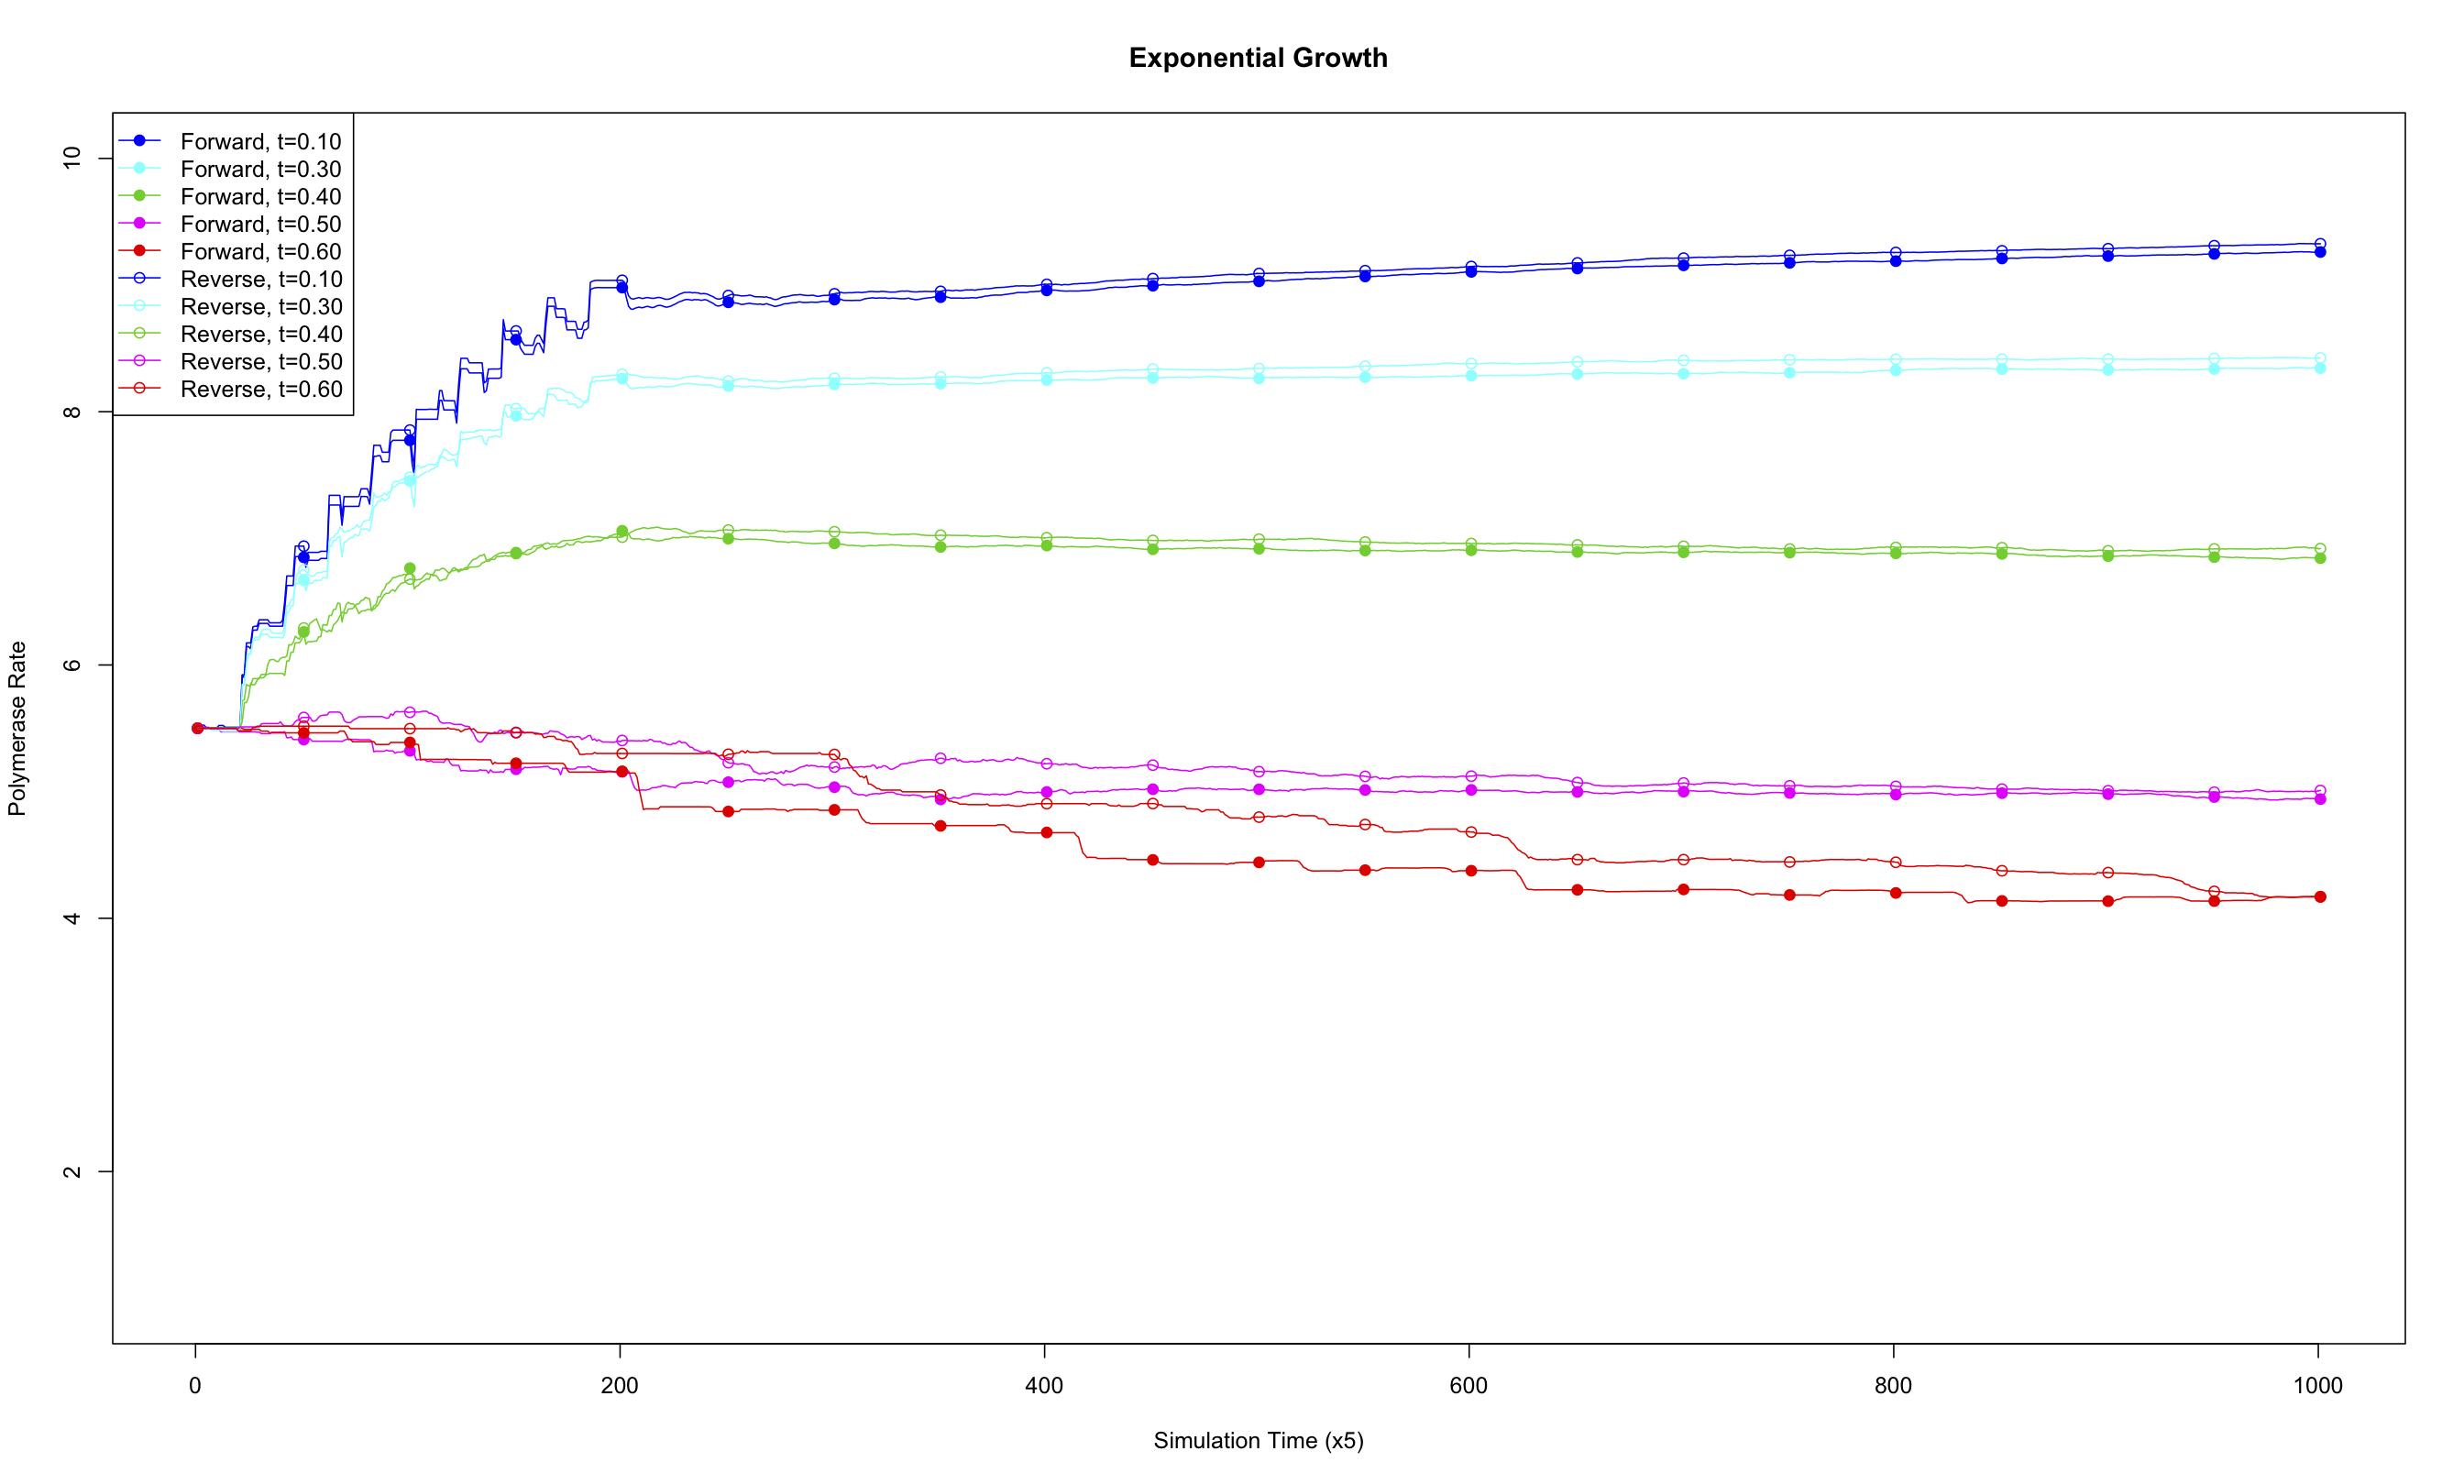
\includegraphics[width=\textwidth]{temp_incr_rate}
	\caption{\textbf{Evolution of polymerase rate for exponentially growing model organisms at various temperatures.} The averages of the polymerase rates for all the model organisms in each environment is plotted for the forward polymerizing organisms (closed circles) and reverse polymerizing organisms (open cicles). The simulation time steps are plotted on the abscissa (each unit represents 5 simulation time steps).}
	\label{fig:temp_incr_rate}
\end{figure}

In each of the experiments performed up to this point, forward or reverse organisms were allowed to grow in isolation. In order to gain some insight into the dynamics of polymerase evolution, it is necessary to set these two classes of model organisms in competition with each other. When considering the competition of organisms, there are two domains which are interesting to probe. The first is the competition of the organisms as they explore a new ecological niche. That is, the way in which organisms compete during phases of exponential growth. The second is the competition that occurs when an environment is already at its carrying capacity. It would be expected that an evolutionary strategy which results in the most rapid growth should dominate during exponential growth. It is also conceivable that such a strategy might not represent the most efficient use of resources available and therefore might ultimately loose out to a different strategy when growth is limited by resources.

To understand both of these domains, two more sets of experiments were performed. In the first set, the simulation environments were seeded with 10 organisms, 5 each with forward or reverse polymerizing polymerases. Again, in order to avoid unnecessary founder bias in the polymerase rates, a cluster of polymerase rates was included in the starting population. Since the starting population was divided between the two types of model organisms, the starting population consisted of one each of organisms with polymerase rates of 3, 4, 5, 6, or 7 going forward or backward. The experimental conditions are summarized in table~\ref{tab:cluster_growth}. Simulations were carried out at various temperatures in order to additionally probe the effect that temperature would have on the competition between the two organism types.

\begin{table}
	\begin{center}
		\begin{tabular}[c]{ c | l | l | l | c }
			Experiment & Temp. ($t$) & Max Pop. & Genome Length & Seed organisms \\
			\hline
			& 0.10 & & & 5 forward\\
			& 0.30 & & & (rates: 3, 4, 5, 6, 7)\\
			\#19-23 & 0.40 & 1000 & 1000 & and\\
			& 0.50 & & & 5 reverse\\
			& 0.60 & & & (rates: 3, 4, 5, 6, 7)\\
		\end{tabular}
		\caption{Competitive growth at various temperatures.}
		\label{tab:cluster_growth}
	\end{center}
\end{table}

A plot of how the polymerase rate evolved over time at each temperature is presented in figure~\ref{fig:cluster_growth_rate}. For each temperature condition, the forward rate is represented by the line with closed circles and the reverse rate is represented by the line with open circles. In addition to the way the polymerase rate evolves, it is also important to know how the organisms fared in terms of survival in the face of competition. So, the population of the forward and reverse polymerizing organisms at each temperature is presented in figure~\ref{fig:cluster_growth_num}. Again, the lines with closed circles represent the forward polymerizing organisms and the open circles represent the reverse polymerizing organisms.

\begin{figure}[h]
	\centering
		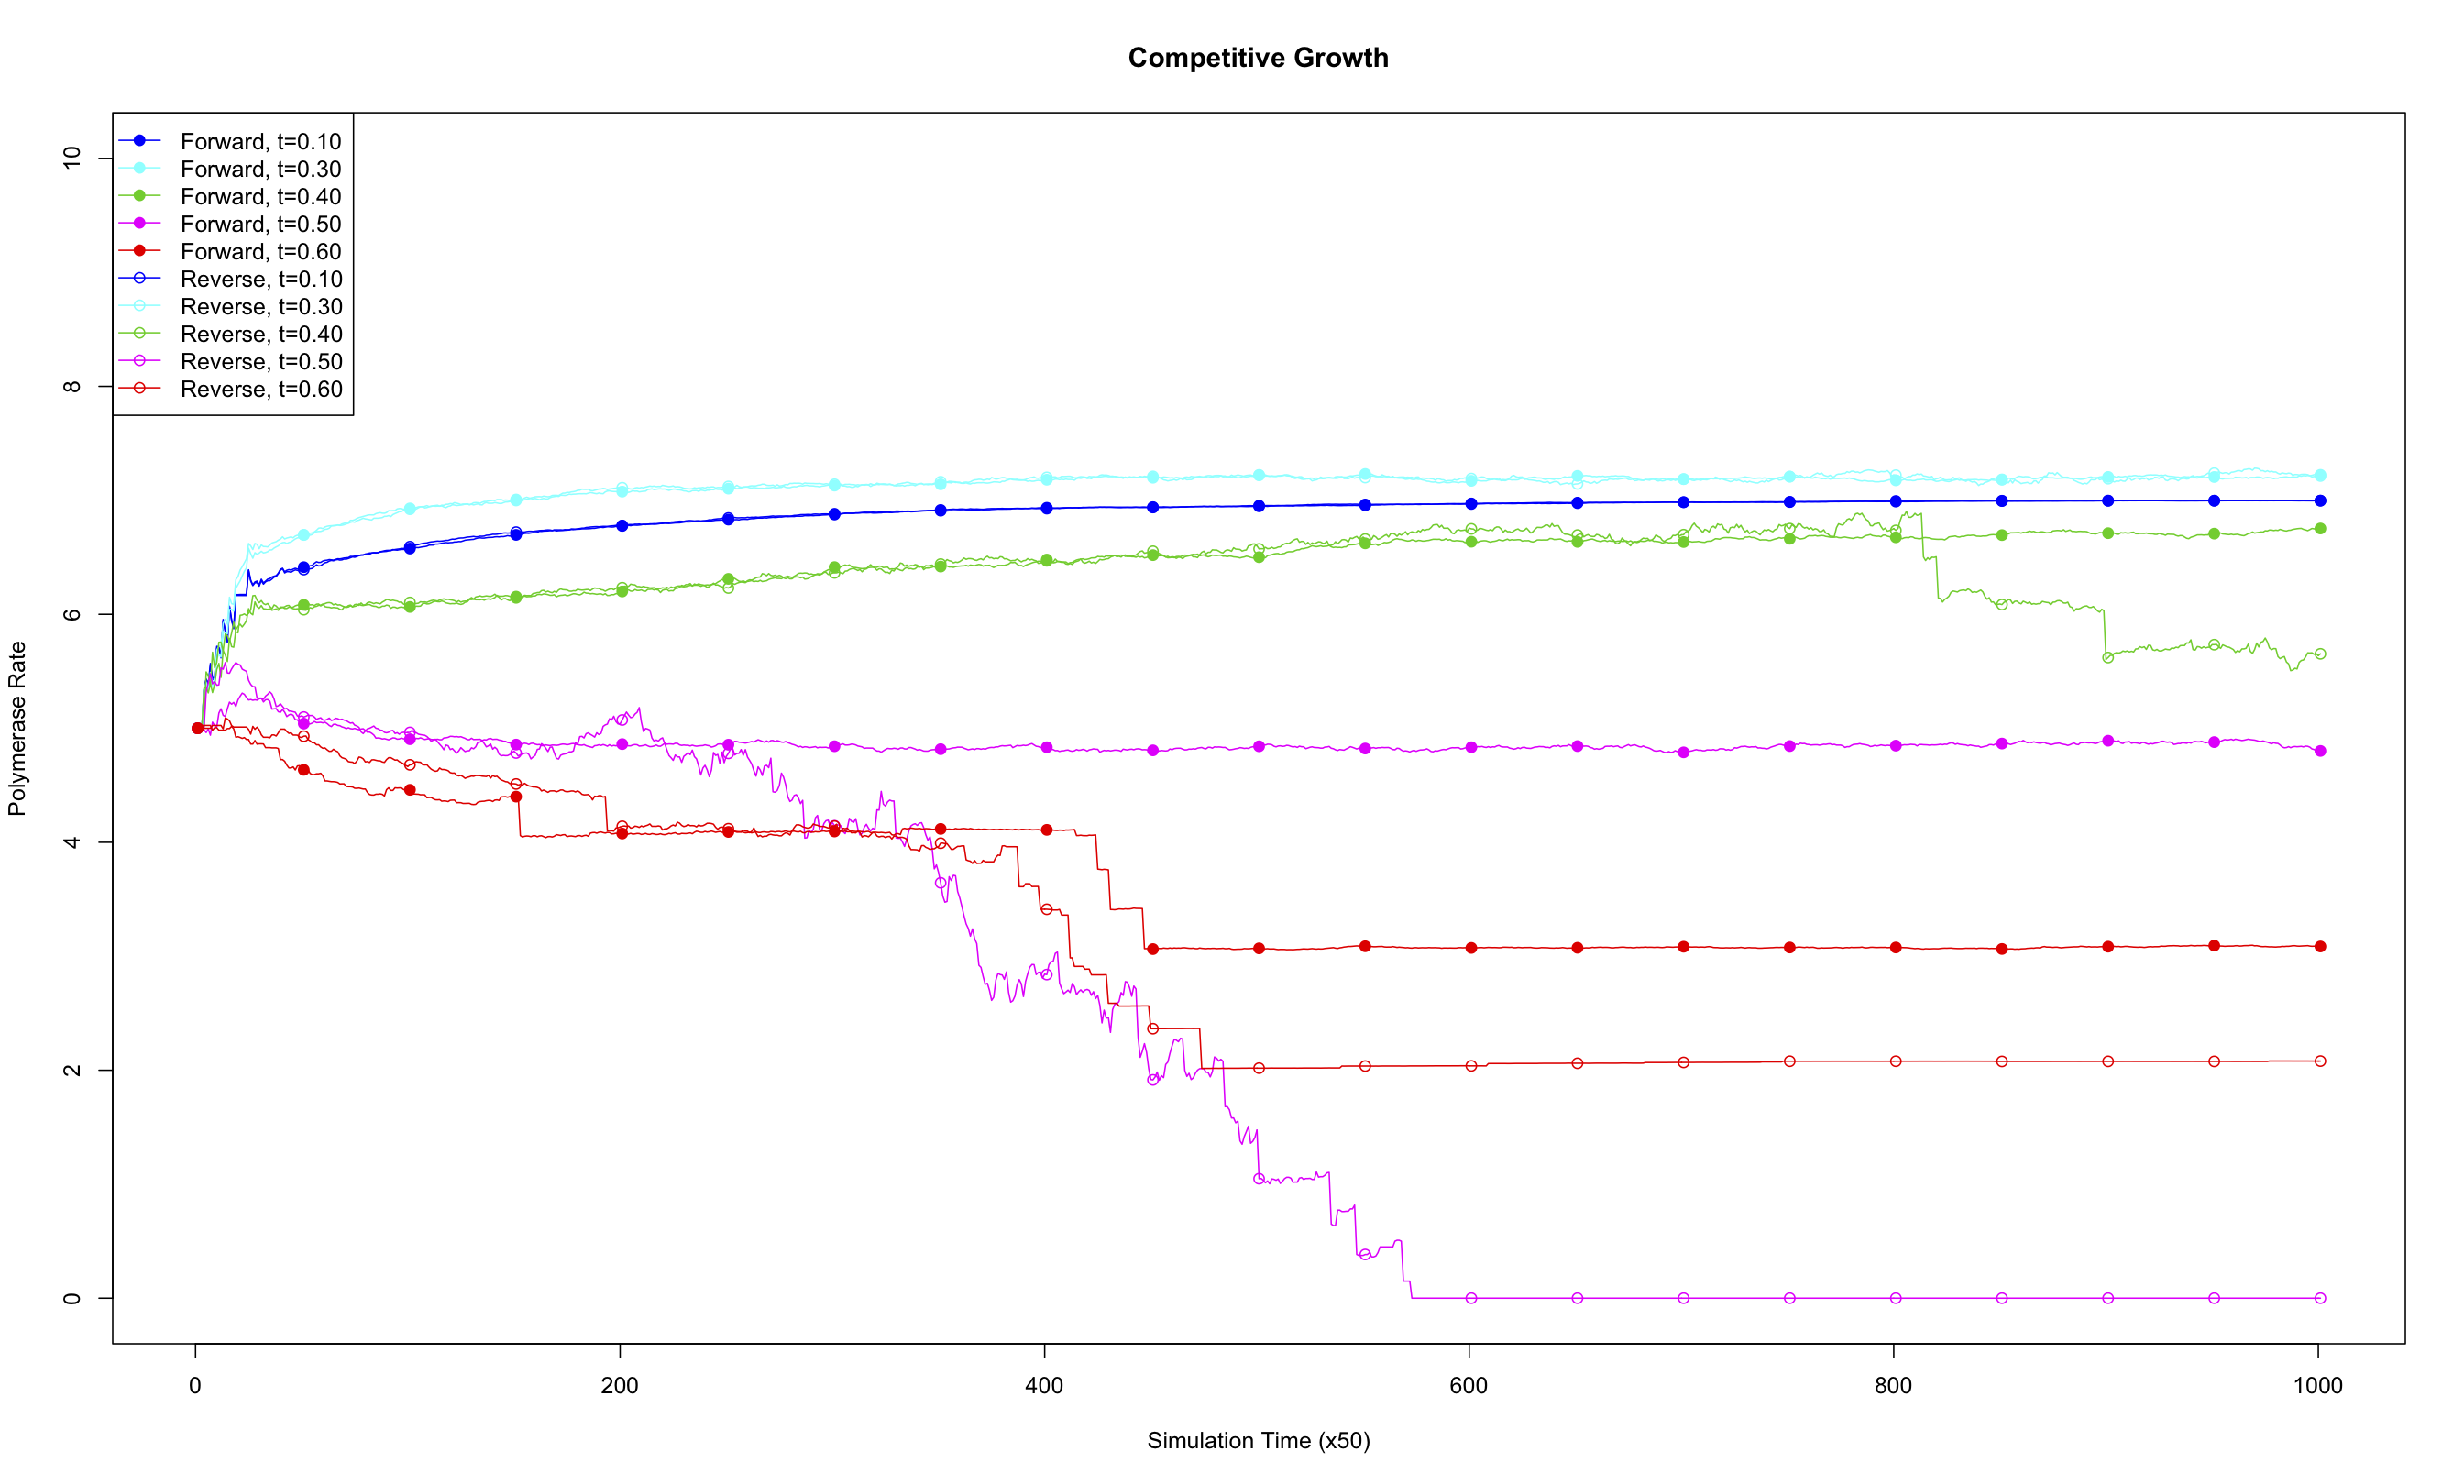
\includegraphics[width=\textwidth]{cluster_growth_rate}
	\caption{\textbf{Competitive evolution of forward and reverse polymerase rates.} The averages of the polymerase rates for all the forward polymerizing organisms (closed circles) and reverse polymerizing organisms (open circles) in each environment is plotted against simulation time. Each unit on the abscissa represents 50 simulation time-steps.}
	\label{fig:cluster_growth_rate}
\end{figure}

\begin{figure}[h]
	\centering
		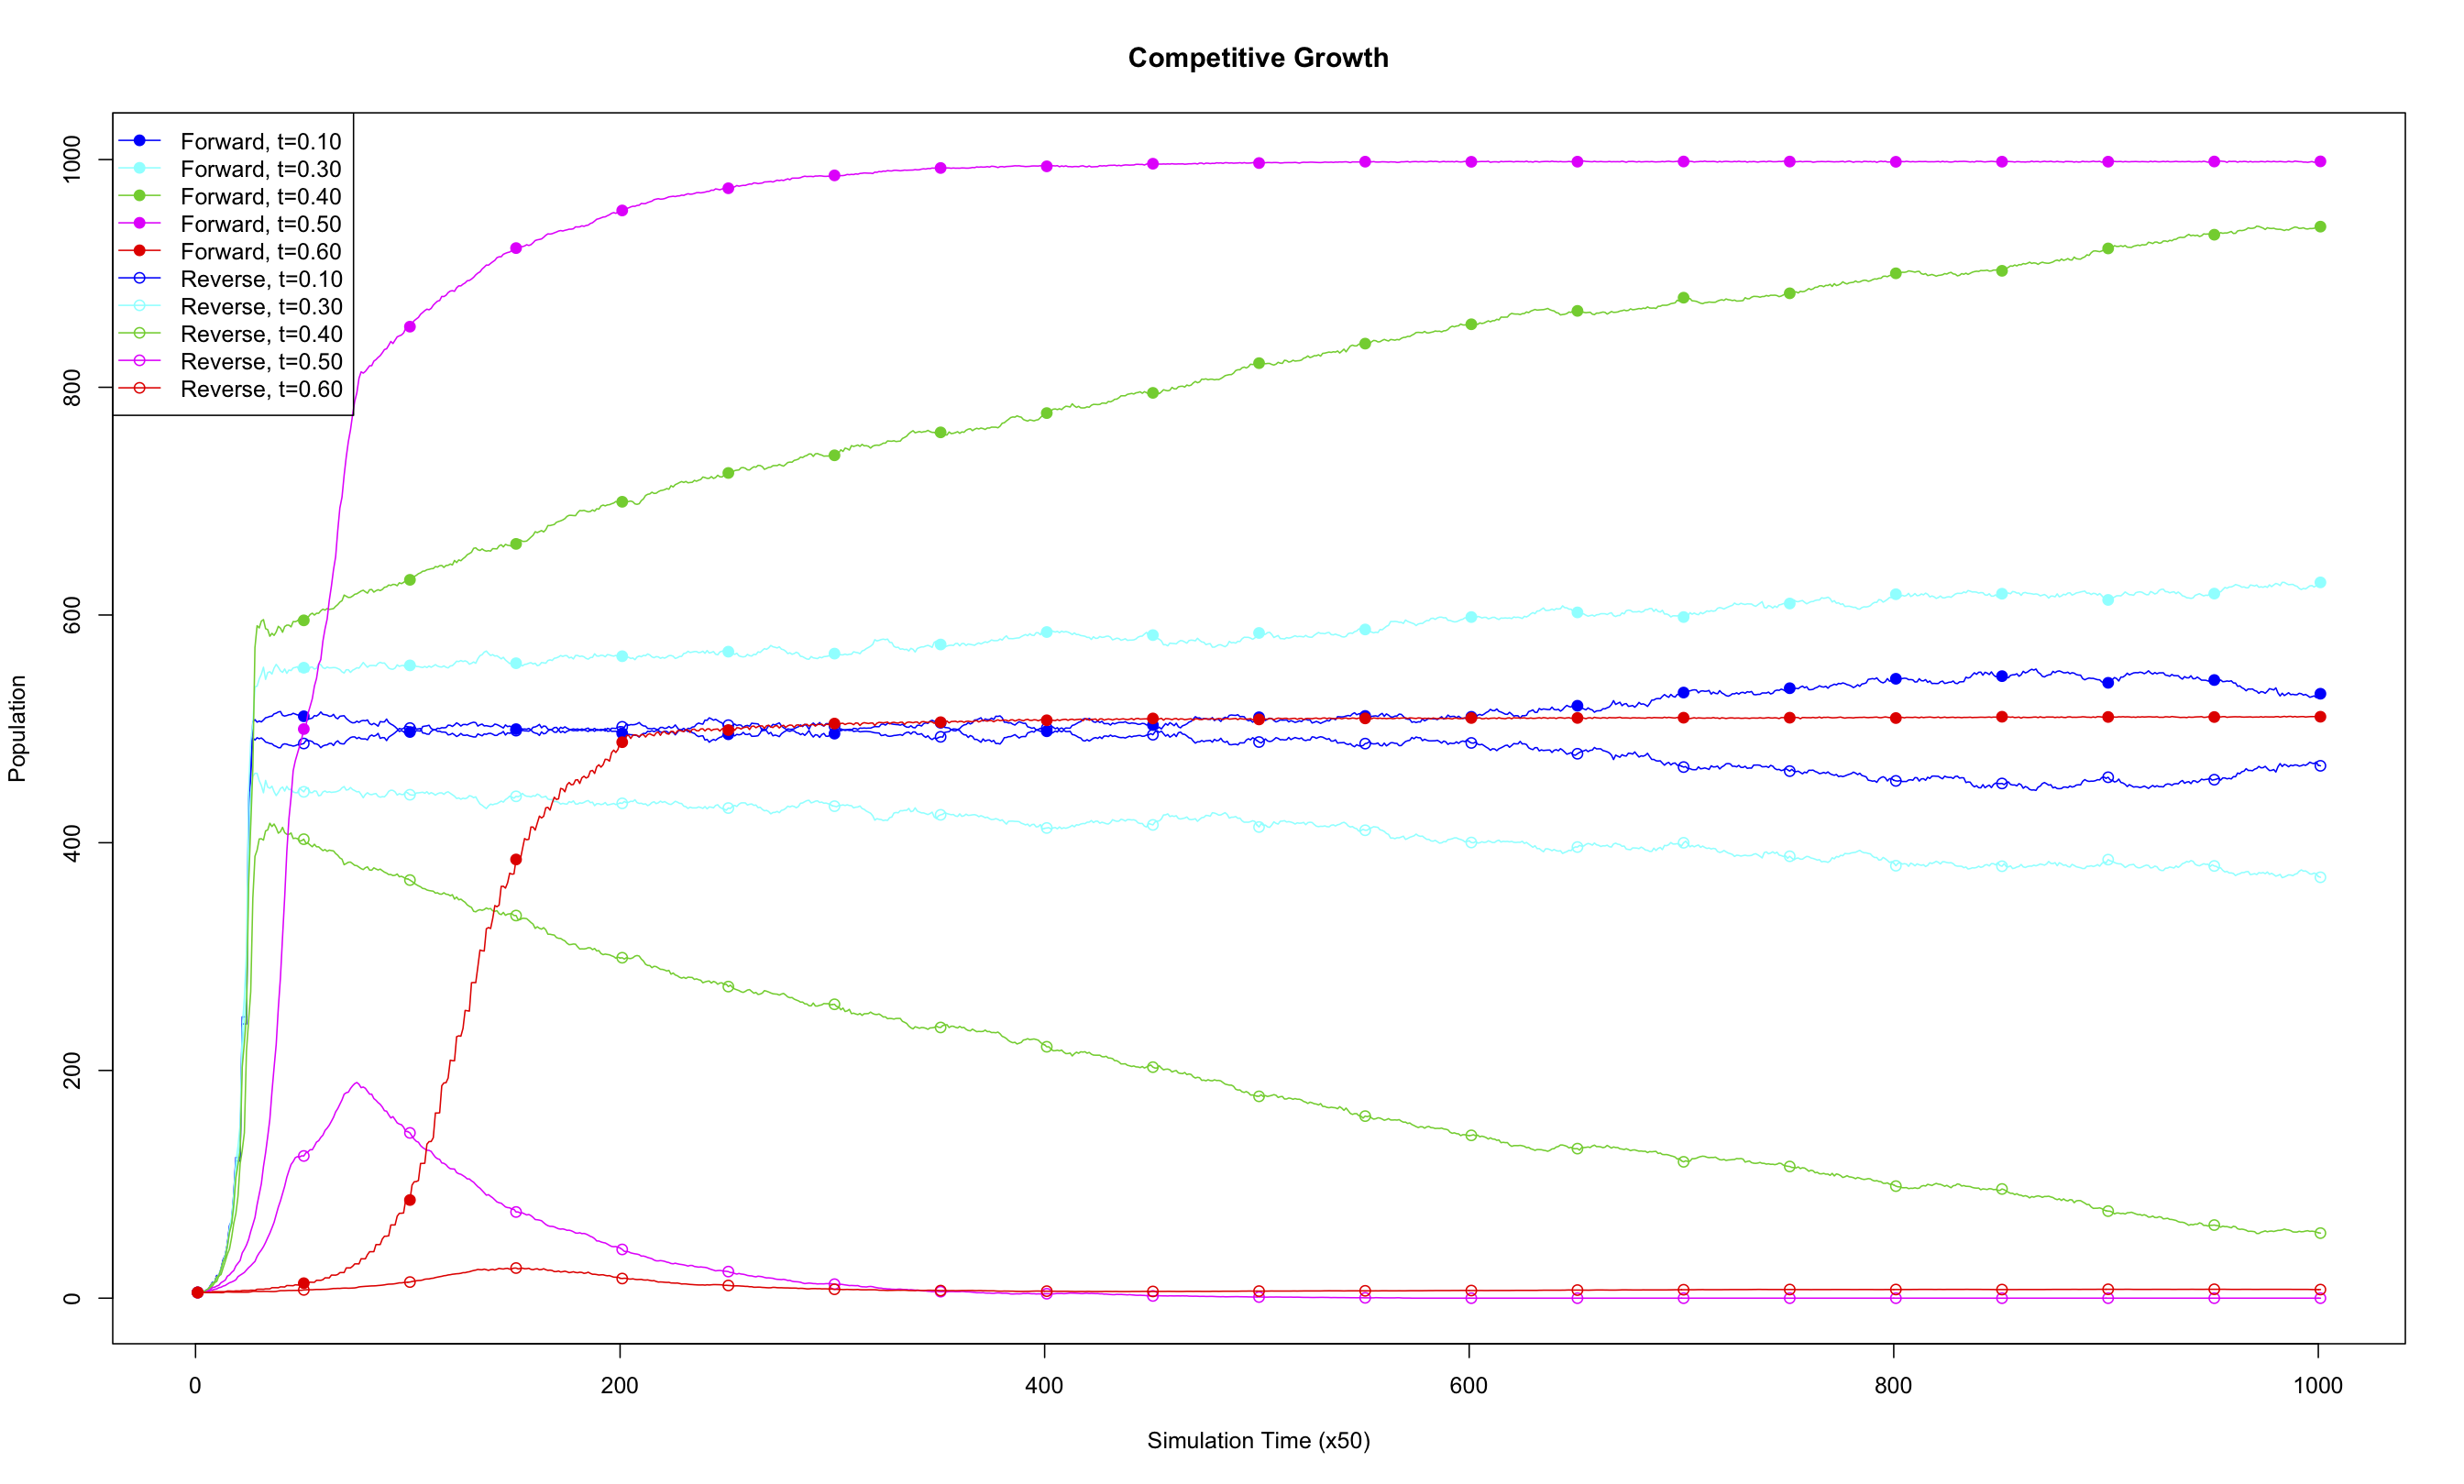
\includegraphics[width=\textwidth]{cluster_growth_num}
	\caption{\textbf{Competitive growth of forward and reverse polymerizing organisms.} The total population of forward polymerizing organisms (closed circles) or reverse polymerizing organisms (open circles) for each environment is plotted against simulation time. Each unit on the abscissa represents 50 simulation time-steps.}
	\label{fig:cluster_growth_num}
\end{figure}

The final experiment consisted of seeding each environment with the maximum population for that environment. This means that each environment, with a carrying capacity of 1000, started with 500 forward polymerizing organisms and 500 reverse polymerizing organisms. Forward and reverse polymerizing organisms were equally distributed between all possible values, 1 to 10, for polymerase rate. The environments were all run at different temperatures. Table~\ref{tab:strict} summarizes the experimental conditions.

\begin{table}
	\begin{center}
		\begin{tabular}[c]{ c | l | l | l | c }
			Experiment & Temp. ($t$) & Max Pop. & Genome Length & Seed organisms \\
			\hline
			& 0.10 & & &\\
			& 0.15 & & &\\
			& 0.20 & & & 500 forward\\
			& 0.25 & & & (rates: 1-10)\\
			& 0.30 & & &\\
			\#24-34 & 0.35 & 1000 & 1000 & and\\
			& 0.40 & & &\\
			& 0.45 & & & 500 reverse\\
			& 0.50 & & & (rates: 1-10)\\
			& 0.55 & & &\\
			& 0.60 & & &\\
		\end{tabular}
		\caption{Competitive growth in a full environment at various temperatures.}
		\label{tab:strict}
	\end{center}
\end{table}

A plot detailing the change in polymerase rate over time is presented in figure~\ref{fig:strict_rate} for the 0.10, 0.30, 0.40, 0.50, and 0.60 simulation temperature experiments. As in figure~\ref{fig:cluster_growth_num}, the forward values are represented with closed circles and the reverse with open circles. The number of forward and reverse polymerizing organisms in the environments at the same subset of simulation temperatures is presented in figure~\ref{fig:strict_num}. Additionally, since the primary goal of these experiments is to determine under what, if any conditions, the population of reverse polymerizing organisms drops to zero, the number of reverse polymerizing organisms at each of the simulation temperatures is presented as figure~\ref{fig:strict_num_rev}.

\begin{figure}[h]
	\centering
		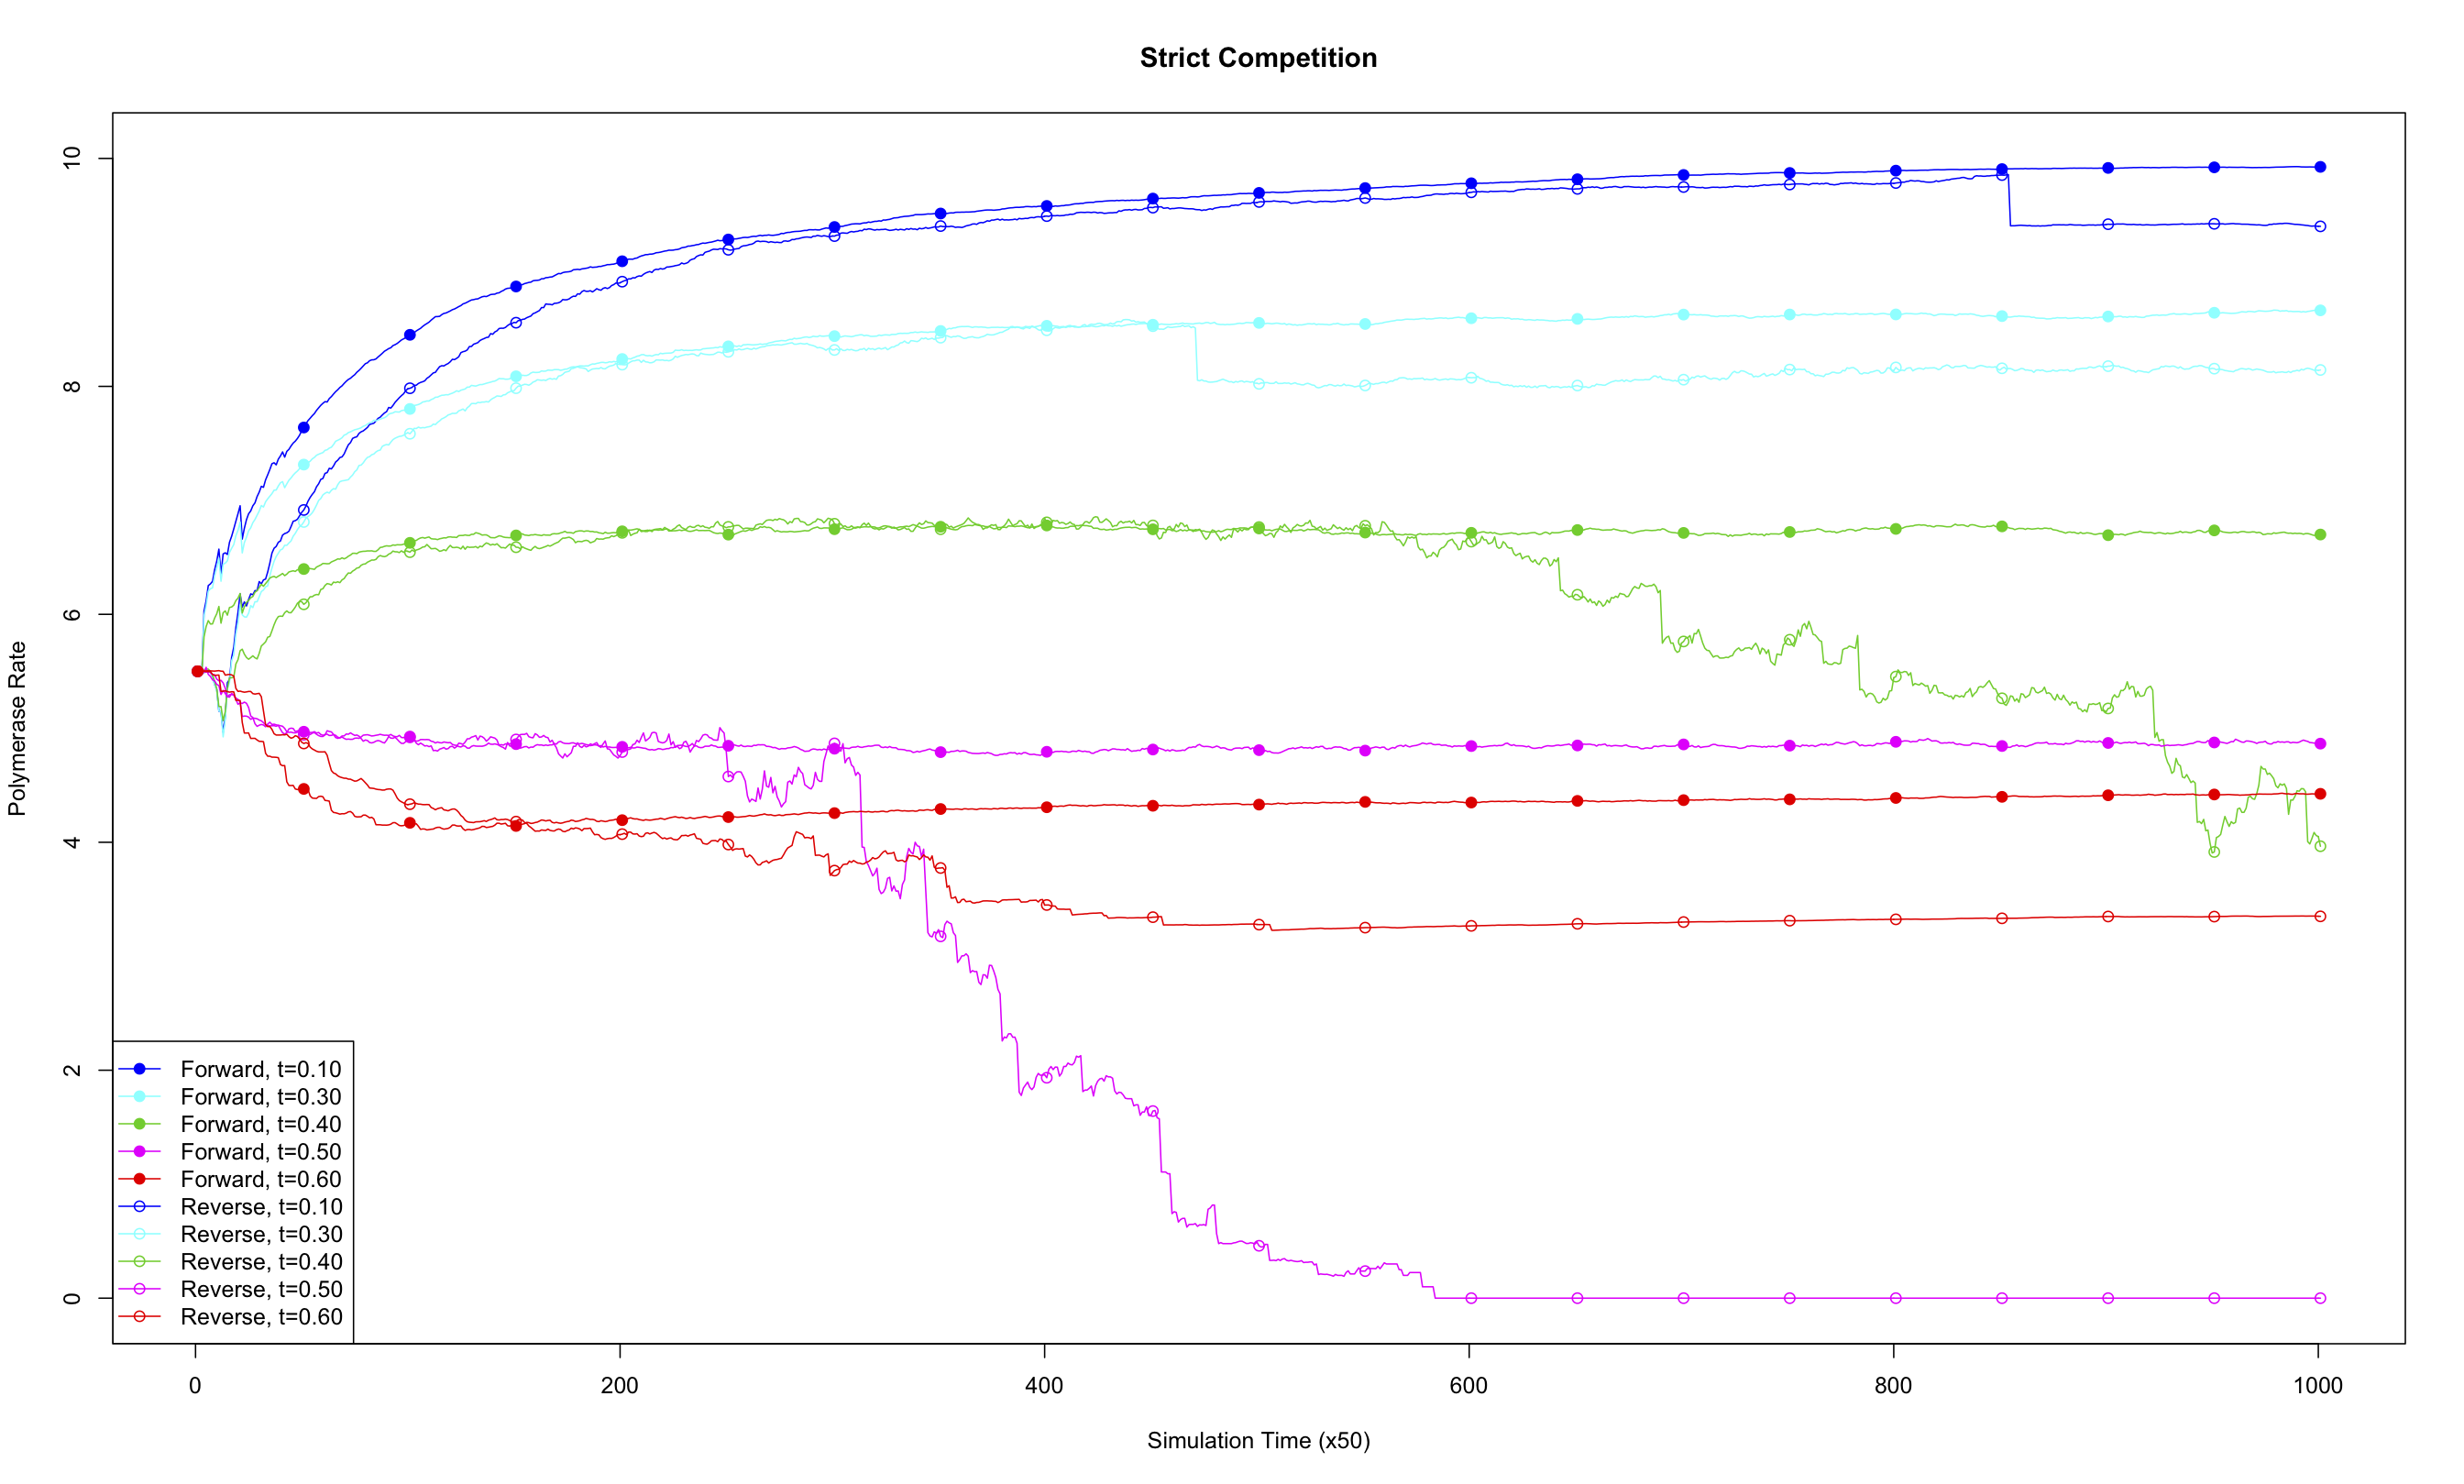
\includegraphics[width=\textwidth]{strict_rate}
	\caption{\textbf{Competitive evolution of polymerase rate for forward and reverse polymerizing organisms in a full environment.} The average of the polymerase rates for all of the forward polymerizing organisms (closed circles) and reverse polymerizing organisms (open circles) in each environment is plotted against simulation time. Each unit on the abscissa represents 50 simulation time-steps.}
	\label{fig:strict_rate}
\end{figure}

\begin{figure}[h]
	\centering
		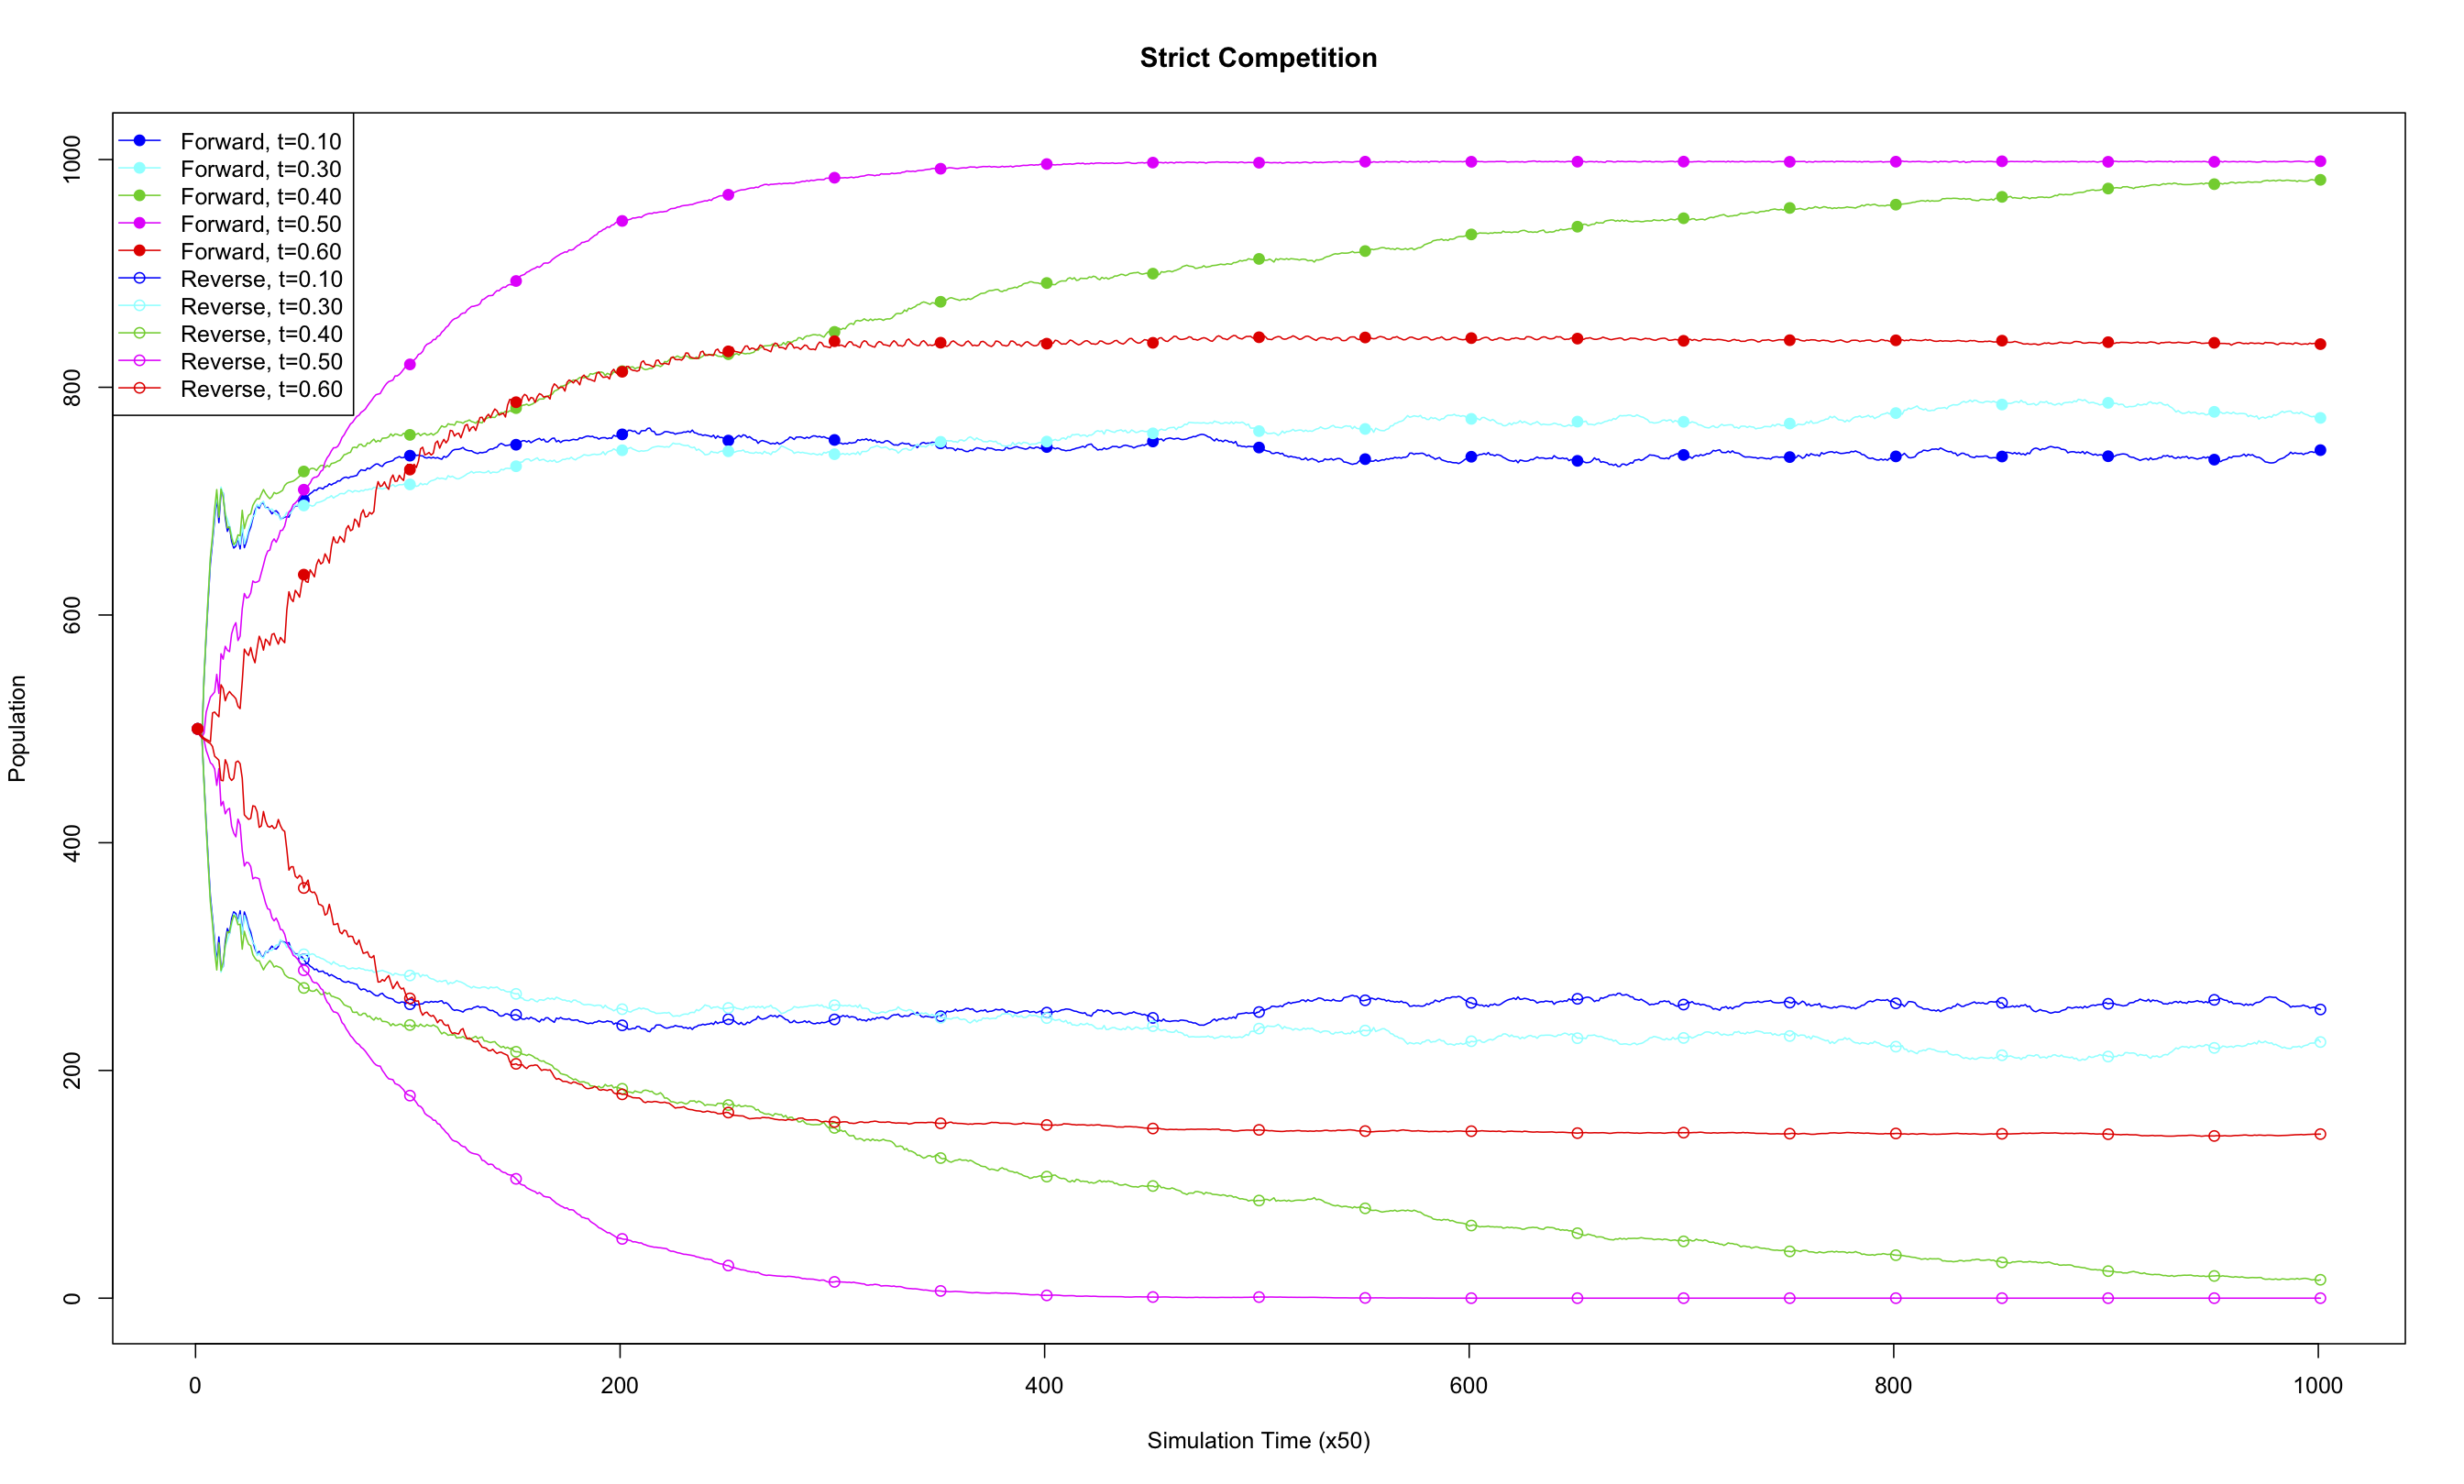
\includegraphics[width=\textwidth]{strict_num}
	\caption{\textbf{Competitive growth of forward and reverse polymerizing organisms in a full environment.} The total population of forward polymerizing organisms and reverse polymerizing organisms in each environment is plotted against simulation time. Each unit on the abscissa represents 50 simulation time-steps.}
	\label{fig:strict_num}
\end{figure}

\begin{figure}[h]
	\centering
		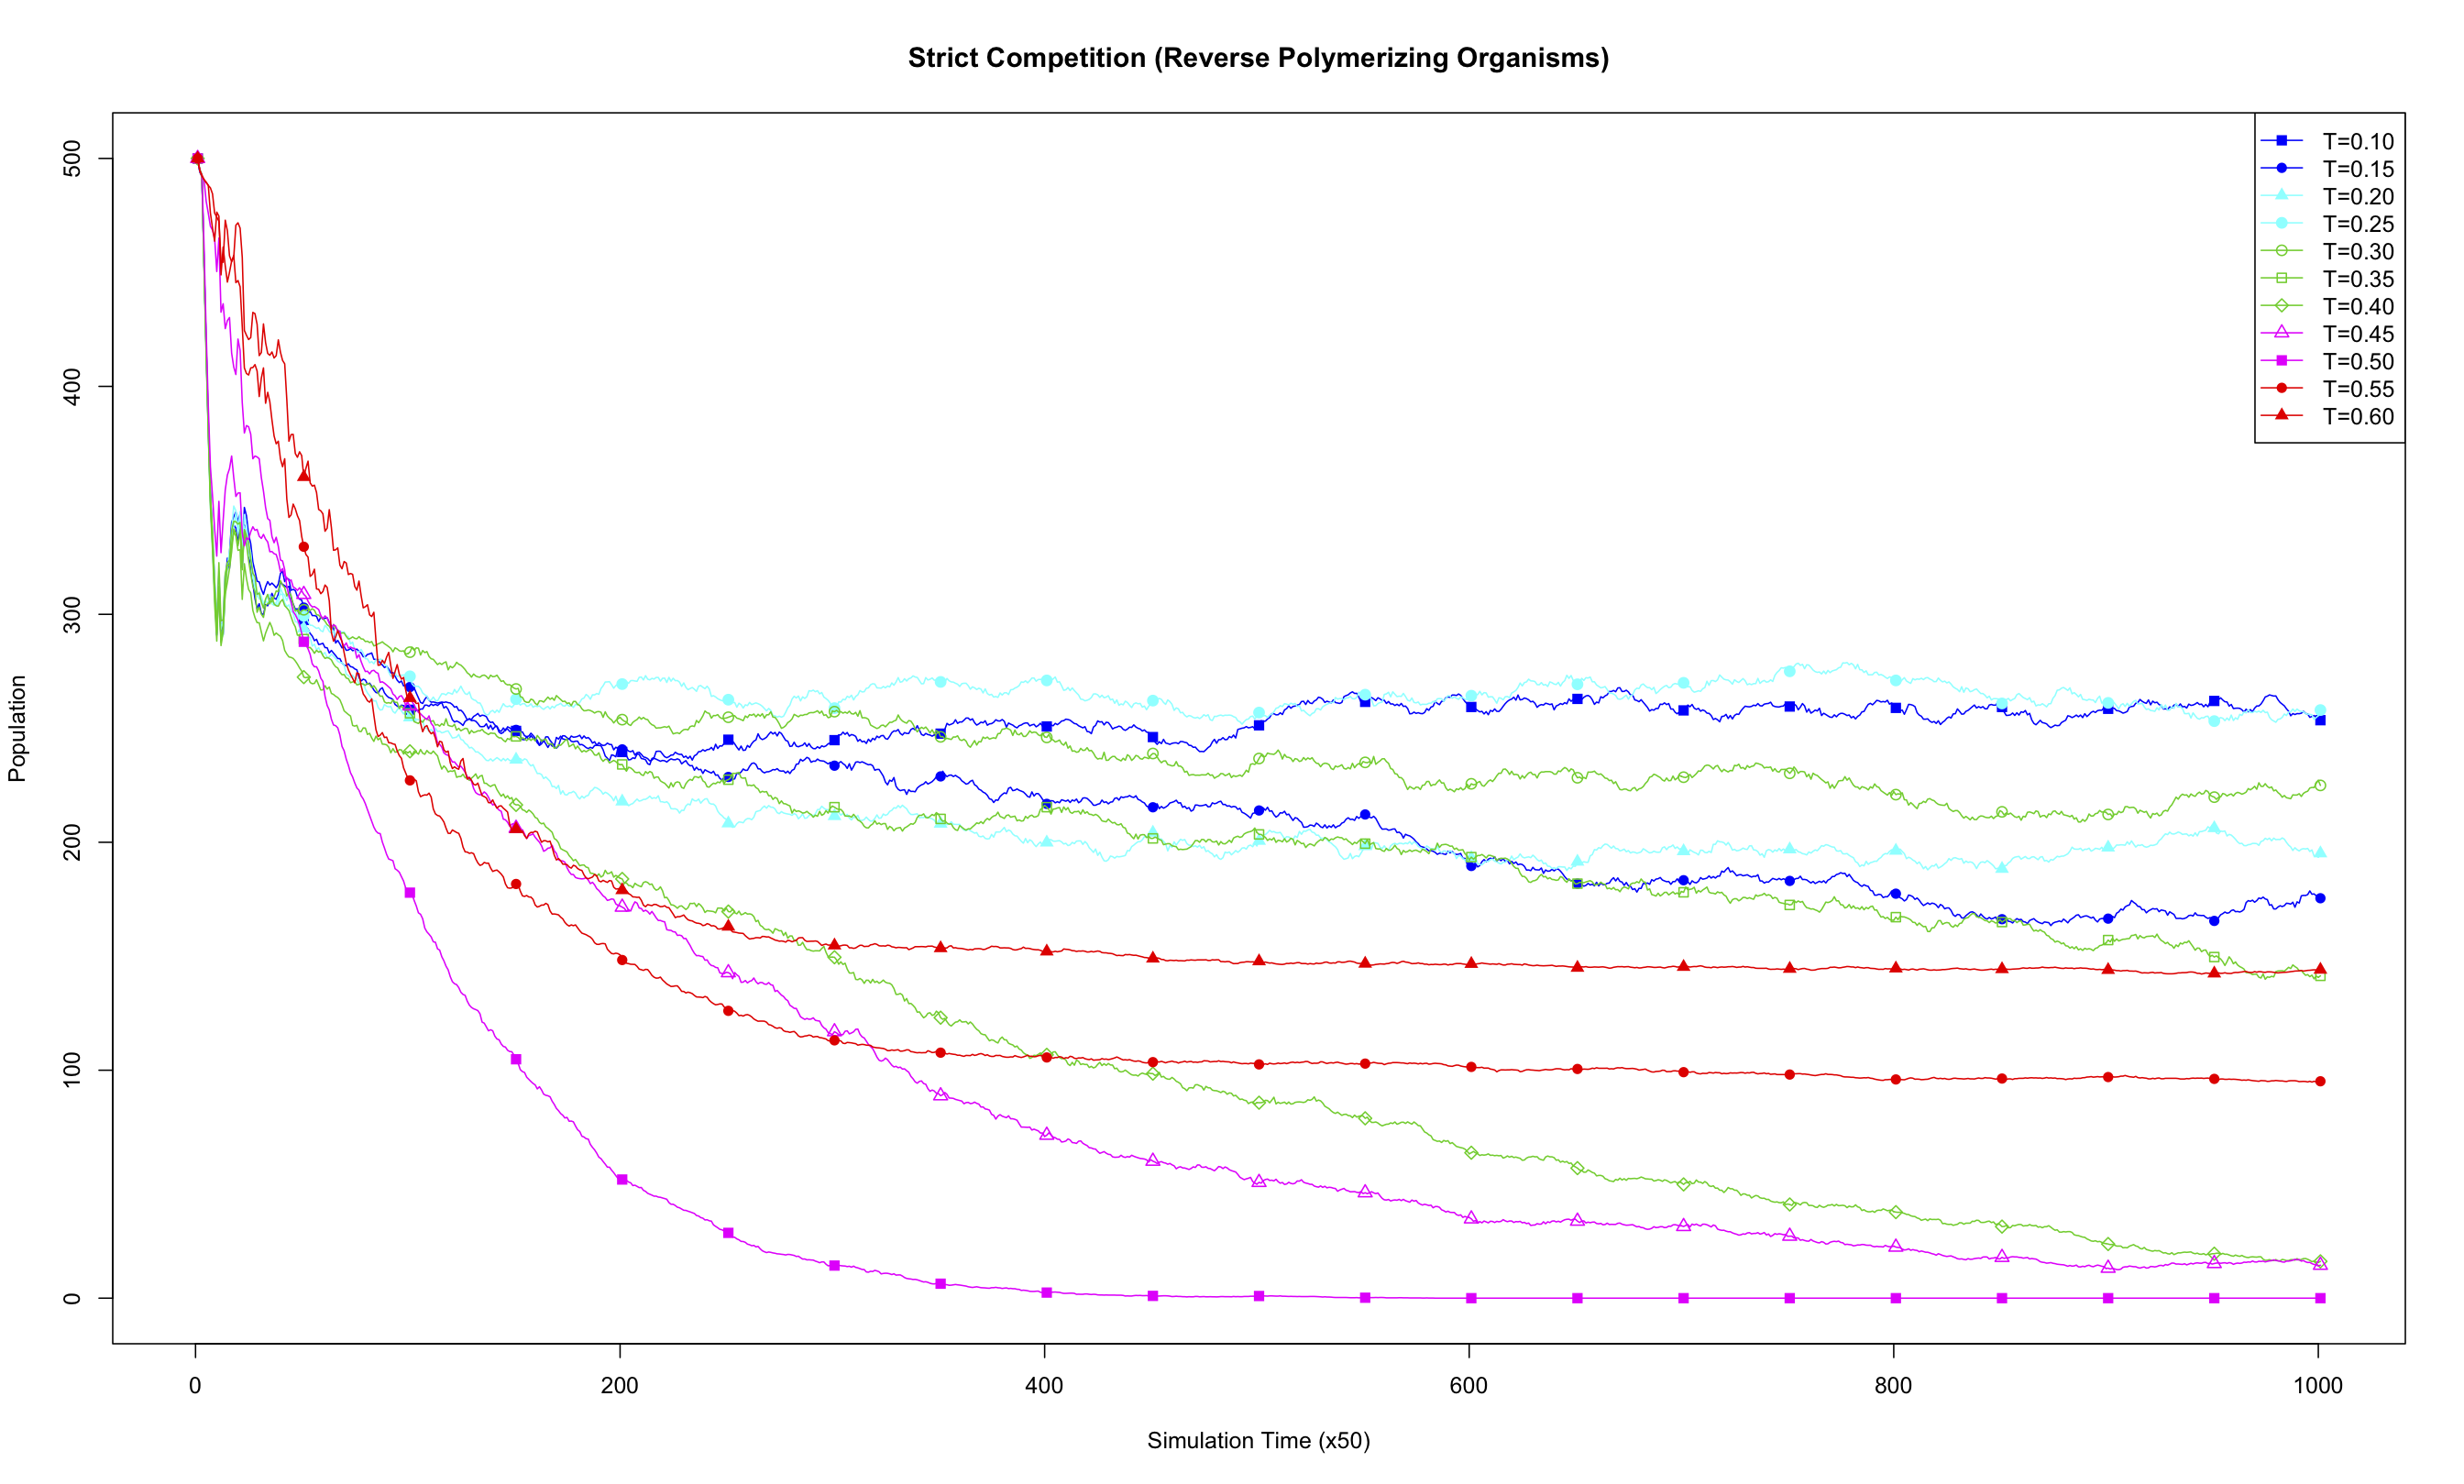
\includegraphics[width=\textwidth]{strict_num_rev}
	\caption{\textbf{Growth of reverse polymerizing organisms under competitive conditions.} The population of reverse polymerizing organisms present in each environment is plotted against simulation time. Each unit on the abscissa represents 50 simulation time-steps.}
	\label{fig:strict_num_rev}
\end{figure}

% chapter experimental_results_of_polymerase_modeling (end)